%!TEX root = ../main.tex
%******************************
%	 Introduction 
%*****************************

\chapter{Introduction}  

\vspace{-1cm}

\graphicspath{{"../../Dropbox (Cambridge  University)/Figures_for_thesis/Introduction/"}}

\begin{Abstract}
\hspace{-5mm} The intrinsic stochasticity of biochemical reactions introduces phenotypic heterogeneity in seemingly homogeneous populations of cells. This phenomenon has been widely studied in prokaryotic and eukaryotic systems and the functional role of phenotypic variation in development, health and disease is the subject of ongoing research. Biological noise, a term to describe molecular variability between individual cells, arises from different sources in homogeneous cell populations. Intrinsic noise summarises stochastic differences in transcription and translation between individual genes \citep{Elowitz2002, Raser2004, Sanchez2013}. Extrinsic noise on the other hand arises when cells reside in different cellular states (e.g.~cell cycle, cell-to-cell signalling and metabolism)  \citep{Zopf2013, Iwamoto2016, Kiviet2014}. Recent technological advances allow the in depth analysis of biological noise in cell populations. Imaging methodologies \citep{Moffitt2016a} and single-cell “omics” techniques \citep{Bock2016} permit the quantification of thousands of mRNA species, the genomic sequence, its epigenetic modification, and selected sets of proteins per cell. Moreover, the development of multi-omics technologies introduced the possibility to link cell-to-cell variation between multiple regulatory layers across individual cells \citep{Macaulay2017}. With the emergence of \gls{scRNA-Seq} technologies, new computational strategies to quantify noise were introduced \cite{Brennecke2013, Vallejos2015, Kolodziejczyk2015cell, Buettner2015, Fan2015a, Richard2016}. Applying high-throughput scRNA-Seq to mammalian systems characterised the functional role of biological noise in healthy as well as diseased contexts. Recent studies have described changes in noise levels at different stages during embryonic development, which hints at stochastic contributions to early cell fate decisions \citep{Goolam2016, Mohammed2017, Ohnishi2014}. On the one hand, phenotypic variation in immune cells, possibly driven by transcriptional noise, increases cellular plasticity and facilitates the population response to pathogens \citep{Shalek2014, Kellogg2015a}. On the other hand, genetic and non-genetic heterogeneity within cell populations was described as driver for cancer development \citep{Marusyk2012} and disrupts immune responses in aged animals \citep{Martinez-jimenez2017, Enge2017}. Here, I introduce noise as an inherent feature of biological system and discuss its positive and negative consequences in cell populations. Furthermore, I outline recent developments of single-cell sequencing and imaging technologies and comment on robust approaches for quantifying biological noise. Finally, I will summarise Bayesian inference as a powerful statistical framework to model transcriptional noise from \gls{scRNA-Seq} data.
\end{Abstract}

\newpage

% Include different main sections of the introduction
%!TEX root = ../intro.tex
%******************************
%	 Biological noise 
%*****************************

\section{Biology of expression noise} 

Biological noise is defined as measurable differences in \gls{mRNA} or protein abundance across homogeneous cell populations (see \textbf{Box 1}). 
%Predominantly, scRNA-Seq technologies, single molecule fluorescence in situ hybridization (smFISH) or fluorescence reporter assays were used to measure the variation in mRNA or protein abundance. 
All cellular systems are exposed to varying levels of noise and employ strategies to make use of or cope with this source of variation. The sources and consequences of biological noise have been studied in an array of viral, prokaryotic and eukaryotic systems while its functional role is controversially discussed depending on the system \citep{Raj2010, Balazsi2011, Eldar2010}. It is crucial to differentiate between unicellular organisms (prokaryotes, viruses, and yeast) in which mainly positive effects of biological noise are described and higher, multicellular eukaryotic systems where biological noise either benefits or obstructs cellular function depending on the tissue type and health state.\\

\begin{Comment}
\textbf{Box 1: Defining biological noise}\\
\small
Biological noise in cell populations arises from stochastic effects on transcription and translation that propagates to form cell-to-cell phenotypic differences. To define noise, one needs to distinguish between different sources of cell-to-cell variability in multiple measurable factors. On the broadest level, differences between single cells in a population can arise from structured (also termed “deterministic” in Marusyk \emph{et al.}, 2012 \citep{Marusyk2012}) and unstructured sources (similar as in Singer \emph{et al.}, 2014 \citep{Singer2014}). When cell populations containing discrete cell-states and/or cell-types are captured \citep{Paul2015, Ibarra-Soria2018, Rosenberg2018}, measuring cell-specific features results in the detection of non-stochastic but rather correlated (structured) differences between individual cells. In cell populations where correlated features do not allow the detection of groups (unstructured variation), continuous processes (e.g.~differentiation) can be the dominating source of cell-to-cell phenotypic variability \citep{Dahlin2018}. Computational approaches allow the detection of these trajectories (e.g.~via principal component analysis or pseudotime inference \citep{Trapnell2014, Angerer2015}). Here, I therefore define biological noise as unstructured, phenotypic cell-to-cell differences independent of measurement errors. 
As previously introduced \citep{Elowitz2002}, biological noise can broadly arise from intrinsic and extrinsic sources. Intrinsic noise originates from stochastic biochemical effects within one cell that directly influences gene-specific expression \citep{Swain2002} (e.g.~transcription factor binding dynamics). Extrinsic noise on the other hand introduces co-expression across multiple genes (also in a pathway specific manner \citep{Raser2010}) due to differences in cell-specific factors such as stress response, mitochondrial maintenance, amino-acid synthesis \citep{Stewart-Ornstein2012} or cell-cycle \citep{Zopf2013}. Intrinsic noise can therefore be measured as expression differences between co-regulated genes in one cell while extrinsic noise is measured as co-regulated variance in gene sets across all cells.\\
\end{Comment}

\subsection{Bet-hedging in unicellular systems}

Biological noise has been described to trigger the differential decision between latency and replication in viruses such as \Gls{HIV} and the \gls{lambdaPhage}. In the case of the \gls{lambdaPhage}, infected cells either reside in a lysogenic state where the genetic material of the virus is transmitted to daughter cells without inducing cell death or a lytic state where the virus destroys the host cell \citep{Lieb1953}. Previous studies have shown that the lysis-lysogeny switch in \gls{lambdaPhage} is driven by intrinsic and extrinsic noise \citep{Arkin1998, St-Pierre2008}. This idea has been extended by Zeng \textit{el al.}, 2010 where the lysis-lysogeny switch does not depend on a single noise-driven decision but on the sum of all individual phages per cell \citep{Zeng2010}. A similar ‘bet-hedging’ strategy, a probabilistic decision between multiple states, exists for \Gls{HIV} infection. Upon infection, \Gls{HIV} either rapidly replicates or resides in a long-lived latent state from which the virus can switch to replication \citep{Weinberger2015}. It has been shown that combining noise-enhancing and activating drugs shifts latent viruses into the active-replication state that can be targeted by anti-retroviral therapeutics \citep{Dar2014}. \\

In unicellular organisms, phenotypic heterogeneity facilitates the commitment to alternative cell states in cases of stress (e.g.~nutrient deprivation, temperature fluctuations). For example, \Gls{Bsubtilis} either commits to sporulation or competence upon starvation or DNA damage. Sporulation describes an irreversible process during which vegetative growth ends and the cell forms endospores that survive the altered environment. Competent bacteria on the other hand can take up DNA from these endospores to repair DNA damage \citep{Schultz2009}. The probabilistic and transient activation of competence in a sub-population of \Gls{Bsubtilis} cells is modulated by fluctuations in the competence regulators ComK and ComS. An excitable system of negative and positive feedback loops controls the number of cells that reversibly commit to competence while other cells irreversibly execute sporulation \citep{Suel2006}. Noise in the process of transferring phoshporyl groups across a cascade of regulators maintains a constant probability for cells to commit to sporulation under nutrient deprived conditions \citep{Russell2017}. A similar phenomenon is observed in \Gls{Ecoli} populations exposed to antibiotics where a pre-existing phenotypic heterogeneity allows some cells to resist antibiotic treatment. Once regrown, these cells remain sensitive to the antibiotic \citep{Balaban2004}. \\

Similar to phenotypic heterogeneity in unicellular prokaryotes, transcriptional noise facilitates the switching between mating phenotypes in yeast upon exposure to pheromones \citep{Paliwal2007}. Comparably, commitment to utilizing galactose as nutrient source is a cell fate transition, which is facilitated by stochastic gene expression\cite{Acar2008}. \\ 

\newpage

\subsection{Development and differentiation}

Similar to bet-hedging strategies in unicellular organisms, noise can facilitate the switch between cell states and the probabilistic induction of differentiation processes \citep{Eldar2010, Chang2008}. It has been shown that transcriptional noise increases throughout differentiation \citep{Stumpf2017} and development \citep{Antolovic2017}. Dissecting differentiation processes of hematopoetic progenitor cells revealed an increase in transcriptional noise directly before cell fate decisions are made \citep{Mojtahedi2016, Richard2016}. Once committed, differentiating cell populations collapse in variability and move towards a new attractor state. This process is aided by variable patterns in DNA methylation states that lock cells in a terminal differentiated state \citep{Jenkinson2017}. \\

Studies of recent years have shown that stochasticity in expression is a crucial driver for early (pre-implantation) embryonic development and prior to gastrulation \citep{Dietrich2007}. As early as the 4-cell stage embryo, targets of master pluripotency markers \Gls{Oct4} and \Gls{Sox2} are heterogeneously expressed.  This is caused by heterogeneous methylation patterns of \Gls{H3R26} induced by \Gls{Carm1}, which in turn facilitates the binding of Oct4 and Sox2 to induce pluripotency. Cell with unmethylated H3R26 differentiate towards the extra-embryonic trophoectoderm while pluripotent cells form the inner cell mass \citep{Goolam2016}. Once the cells compact at the 16-cell stage at \Gls{E} 3.5, cells of the \gls{ICM} stochastically express genes to initiate heterogeneity within the cell population. Fgf4 driven signal reinforcement controls this heterogeneity to form a salt-and-pepper like cell state pattern at E3.5. Positional information and the establishment of gene regulatory networks facilitate the segregation of the epiblast and primitive endoderm lineage \citep{Ohnishi2014}. In line with this, scRNA-Seq revealed high levels of noise in the uncommitted inner cell mass at E3.5 (16-cell stage) in comparison to the E4.5 committed epiblast. Noise levels increase again upon exit from pluripotency in the E6.5 epiblast while cells of the primitive streak at E6.5 synchronize their expression patterns and noise is reduced \citep{Mohammed2017}.\\

While pluripotent stem cells in the mouse embryo commit irreversibly to cell lineages during development, \emph{in vitro} cultured \glspl{mESC} reside in a self-renewing, metastable state \citep{Hayashi2013}. Heterogenity within the cell population depends on the growth conditions that the cells are being kept in. Transcription factor heterogeneity, especially of the pluripotency regulator Nanog, is highest in \Gls{LIF}/serum grown cells and allows the Nanog-negative cells to commit to differentiation lineages \citep{Chickarmane2012, Torres-Padilla2014}. Heterogeneously expressed genes that show a bimodal distribution in expression counts correlate with each other indicative for the presence of distinct states in mESCs. These distinct states show differences in promoter methylation patterns introducing the role of epigenetic modifications to maintain heterogeneity in mESCs \citep{Singer2014a}. In-depth analysis of mESCs grown in different media (serum, 2i and a2i) shows the presence of three distinct cell states in the serum grown cells. mESCs grown in 2i media show less variability in pluripotency markers but higher heterogeneity in cell-cycle related genes \citep{Kolodziejczyk2015cell}. From the pluripotent ground state, mESCs can differentiate along somatic lineages via specific differentiation events or noise-induced transition between attractor states. Mathematical modelling has shown that mESCs differentiate stochastically through distinct hidden cell (micro-)states within a defined (macro-)state coupled to an increase in variability \cite{Stumpf2017}.\\

In contrast to the beneficial features of noise in stem cell differentiation, stochastic events during \gls{iPSC} reprogramming limit the formation of single iPSCs \citep{Hanna2009, Yamanaka2009}. It has been shown that probabilistic events dominate in an early phase of reprogramming while the transcription of Sox2 induces a later, more deterministic, phase \cite{Buganim2012}. While heterogeneity in gene expression and protein abundance has been characterized to benefit cell commitment and differentiation, other reports propose alternative hypothesis for cell fate decisions where commitment is independent of random fluctuations of transcription factors \cite{Hoppe2016}. Similarly, the increase in noise during development can be counteracted by temporal averaging across noisy transcription events to achieve coordinated tissue responses \citep{Stapel2017}. 

\subsection{Stochasticity in immune responses}

Fast and flexible immune responses are only possible within cell populations that show high plasticity and react to a broad spectrum of stimuli. Stochasticity in cytokine expression leads to phenotypic variability in the \Gls{Th} cell repertoire and increases the effectiveness to respond upon immune stimuli \citep{Schrom2017}. For example, fluctuating expression of lineage defining cytokines \Gls{Ifn}$\gamma$ for Th1 and \Gls{Il} 4 for Th2 in small populations of cells drive the cell population towards a Th1 or Th2 cell fate while most cells co-express the lineage defining transcription factors \Gls{Gata} 3 and \Gls{Tbx21} \citep{Fang2013a, Antebi2013}.\\

Furthermore, Shalek \textit{et al.}, 2014 have shown that upon \Gls{LPS} stimulation a small subset of dendritic cells become activated much earlier than the rest of the cell population while expressing Ifn$\beta$. These early responders support the activation of late responding cells via cell-to-cell communication \citep{Shalek2014}. Likewise, a bimodal (digital) expression of Il2 is detected in T helper cells after immunization where the number of Il2 expressing cells scales with antigen amount. Il2 expressing cells support the activation of surrounding cells via paracrine signaling \citep{Fuhrmann2016}. Similar digital activation processes can be observed in the \Gls{NFkB} signaling pathway. The fraction of cells that activate the this signaling pathway increase with LPS concentration to avoid strong immune activation at low concentrations of a stimulus \citep{Kellogg2015b}.

\subsection{Tissue development and homeostasis}

Coping with the influence of biological noise is important for regulated tissue development and homeostasis. An early study showed that in order to minimize the effect of stochasticity in development, plants express heat-shock protein 90 to stabilize metastable regulators of growth and development \citep{Queitsch2002}. Furthermore, redundancy in the \Gls{Celegans} intestinal gene regulatory network buffers variability in the down-stream master regulator \textit{elt-2}. Once highly connected regulators of this network are removed, phenotypic variation arises from bimodal expression of the otherwise highly expressed \textit{elt-2} \citep{Raj2010}. The cooperation of positive and negative feedback loops in these highly connected regulatory networks ensure robust expression of key developmental genes \citep{Ji2013}. While complex signalling networks reduce noise during tissue development, other models have been proposed in which noise helps to form sharp boundaries between neighbouring domains \citep{Zhang2012}. While contact based adhesion and repulsion in between cells sharpens narrow transition regions, noise-driven cell state plasticity helps narrowing a wider transition region \citep{Wang2017}. Conversely, rearrangements within a population of cells, allows the correction of sensing errors induced by variation in the strength of single cell responses to a signalling gradient \citep{Camley2017}.\\

While the cell division rate within tissues is higher during development, tissue homeostasis is maintained by stochastic events that balance cell division and apoptosis \citep{Ranft2010}. The effect of noise on maintaining tissue homeostasis has been studied in a diverse set of organs. In fat tissue, a complex system of signalling feedback loops controls protein abundance noise to induce differentiation at a low rate but prevents stochastic de-differentiation \citep{Ahrends2014}. To maintain coordination in liver function, longer bursts of short lived mRNAs and polyploidy reduce noise in gene expression \citep{BaharHalpern2015}. Another mechanism to achieve tissue-wide expression responses involves spatial coordination of stochastically expressing cells in the pituitary gland \citep{Featherstone2016}. Spatially constraint signalling events have also been demonstrated to play a role in maintaining colonic crypt cell-type diversity. Per crypt, eight stem cells differentiate into a defined ratio of cell-types. To reduce noise in this process, lateral inhibition within a commitment zone reduces the number of differentiated goblet cells and following slower dispersive migration as well as decreased division rates of goblet cells ensures a distinct 1:3 ratio to enterocytes \citep{Toth2017}.

\subsection{Evolution}

As discussed above, biological noise is beneficial for cell fate commitment while in other settings, noise needs to be reduced to allow coordinated expression in cell populations. During evolution, a trade-off between cellular plasticity, the expression responsiveness during environmental changes, and robust expression formed. Natural selection acts on genetically controlled expansions of quantitative phenotypes, which are derived from biological noise \citep{Eldar2010}. For example, noisy expression of stress response genes allows a cell population to adapt to changing environments \citep{Lopez-Maury2009}. Specifically, the expression of genes controlled by TATA-box containing promoters shows strong divergence between species \citep{Tirosh2006}. To control for robust expression levels once selection becomes stabilizing, noise levels are reduced \citep{Lopez-Maury2009, Eldar2010, Pires2016}. \\

Lehner, 2008 discussed specifically evolutionary selection to minimise noise in genes that show harmful phenotypic effects upon alteration ("dosage-sensitive genes"). These genes show low expression noise to reduce the probability of altered expression and also lower expression divergence between species \citep{Lehner2008}. Furthermore, essential genes tend to cluster in the genome in regions with persistent open chromatin to reduce noise \citep{Batada2007}. In line with this, the promoters of core cellular components show a decoupling between expression plasticity and expression noise which indicates that responsiveness in expression is not a general attribute of high expression noise \citep{Lehner2010a}. \\

In unicellular populations, noise evolutionarily increased as a form of rudimentary regulation \citep{Wolf2015}. As a consequence, phenotypic heterogeneity increases the adaption rate of cell populations to extreme environments \cite{Bodi2017}. Conversely, in multicellular organisms, collections of cells need to respond in a coordinated manner. It has therefore been proposed that nuclear compartmentalization in higher organisms reduces noise by mRNA retention at the nuclear membrane \citep{Battich2013, Stoeger2016}.

\subsection{Cancer}

While biological noise supports the adjustment of cells to new microenvironments, errors in the form of gene mutations induce transitions from healthy cells towards a cancer attractor state\citep{Marusyk2012}. Non-genetic heterogeneity aided by transcriptional noise supports the phenotypic adaption to the new attractor state \citep{Jia2017}. The emergence of non-genetic heterogeneity in tumors is coupled to epigenetic dysregulation that allows the survival of cancer cells \citep{Timp2013}. Furthermore, it has been proposed that genome wide intrasample methylation heterogeneity is increased in Chronic Lymphoitic Leukemia increasing cancer cell plasticity in the search for new attractor states \citep{Landau2014}.\\
Increased variability in expression can also be observed for more aggressive cancer sub-types across multiple patients \citep{Ecker2015}.  An important consequence of biological noise leading to phenotypic heterogeneity in cancer cells is the fractional killing of cell populations upon drug treatment \citep{Flusberg2015}. Noise in proteins mediating TRAIL induced apoptosis leads to the survival of small fractions of cells \citep{Spencer2009}, which could consequently repopulate the tumor environment. Furthermore, the stochastic acquisition of DNA damage upon cisplatin exposure introduces heterogeneity in the up-regulation of p53. Slow up-regulation leads to cell-cycle arrest and inhibits apoptosis while only fast up-regulation leads to cell death. In patient derived melanoma cells, sporadic expression of resistance markers forms a rare cell population that grow into resistant colonies after treatment. While pre-resistant cells do not display epigenetic marks and are therefore close to the non-resistant ground state, treatment induces large epigenetic reprogramming forming stable resistant cancer colonies \citep{Shaffer2017}. \\
Combinatorial therapies have been proposed to reduce variability and fractional killing in cancer cell populations \cite{Paek2016, Roux2015}.

\subsection{Ageing}

Similarly to the onset of cancer, destructive roles of biological noise have been reported during organismal ageing. Previously, it has been debated whether expression noise changes during the lifespan of animals\cite{Bahar2006, Warren2007}. While these initial studies only used small panels of genes, transcriptional profiling of single cells lead to the discovery of a destabilization of the immune activation program in CD4$^+$ T cells due to increased expression noise \cite{Martinez-jimenez2017}. Similarly, transcriptional noise increases with age in human pancreas coupled to an increased stress signature and atypical hormone expression \citep{Enge2017}.\\


\begin{table}[hb	]
\centering
\caption{Positive and negative effects of biological noise on cellular systems}
\label{table:effects_noise}
\begin{tabular}{l l l}
\toprule
System & Friend & Foe \\ 
\midrule
Unicellular organism & Bet-hedging & \\
\midrule
Development and & Probabilistic induction  & \\
differentiation & of cell differentiation & \\
\midrule
Immune response & Plasticity in immune response & \\
 & Control of response strength &   \\
\midrule
Tissue development  & Low cell differentiation rate & Non-uniform development \\ 
and homeostasis &  & Uncontrolled tissue response \\
\midrule
Evolution & Adjustment to  & Non-uniform, stabilizing expression \\ 
& fluctuating environment & Uncontrolled tissue responses \\
\midrule
Cancer &  & Phenotypic adaption to cancer state \\
& & Fractional killing of cancer cells \\
\midrule
Aging &  & Unsynchronized immune response \\
& & Increased stress signatures \\ 
\bottomrule
\end{tabular}
\end{table}

\newpage
%!TEX root = ../intro.tex
%******************************
%	 Sources of expression noise
%*****************************

\section{Sources of expression noise} 

Variability in expression across homogeneous populations of cells arises from intrinsic and extrinsic sources of noise (see \textbf{Box 1}). While intrinsic noise is promoter-specific and therefore induces uncoordinated variation in RNA or protein expression between individual genes, extrinsic noise globally influences gene expression across multiple cells and therefore leads to co-variation across larger set of genes. Here, I give an overview on the different sources of intrinsic and extrinsic noise and discuss their beneficial or disruptive features in biological systems.

\subsection{Intrinsic noise}

Intrinsic noise in cell populations arises from stochasticity in biochemical reactions that lead to the synthesis of mRNAs (transcription) and proteins (translation) within individual cells. Regulatory features on the DNA, epigenetic, transcriptional and translational level influence the strength of intrinsic noise (for an overview see \textbf{Fig.~\ref{fig0:overview_intrinsic}}).

\begin{figure}[!h]
\centering
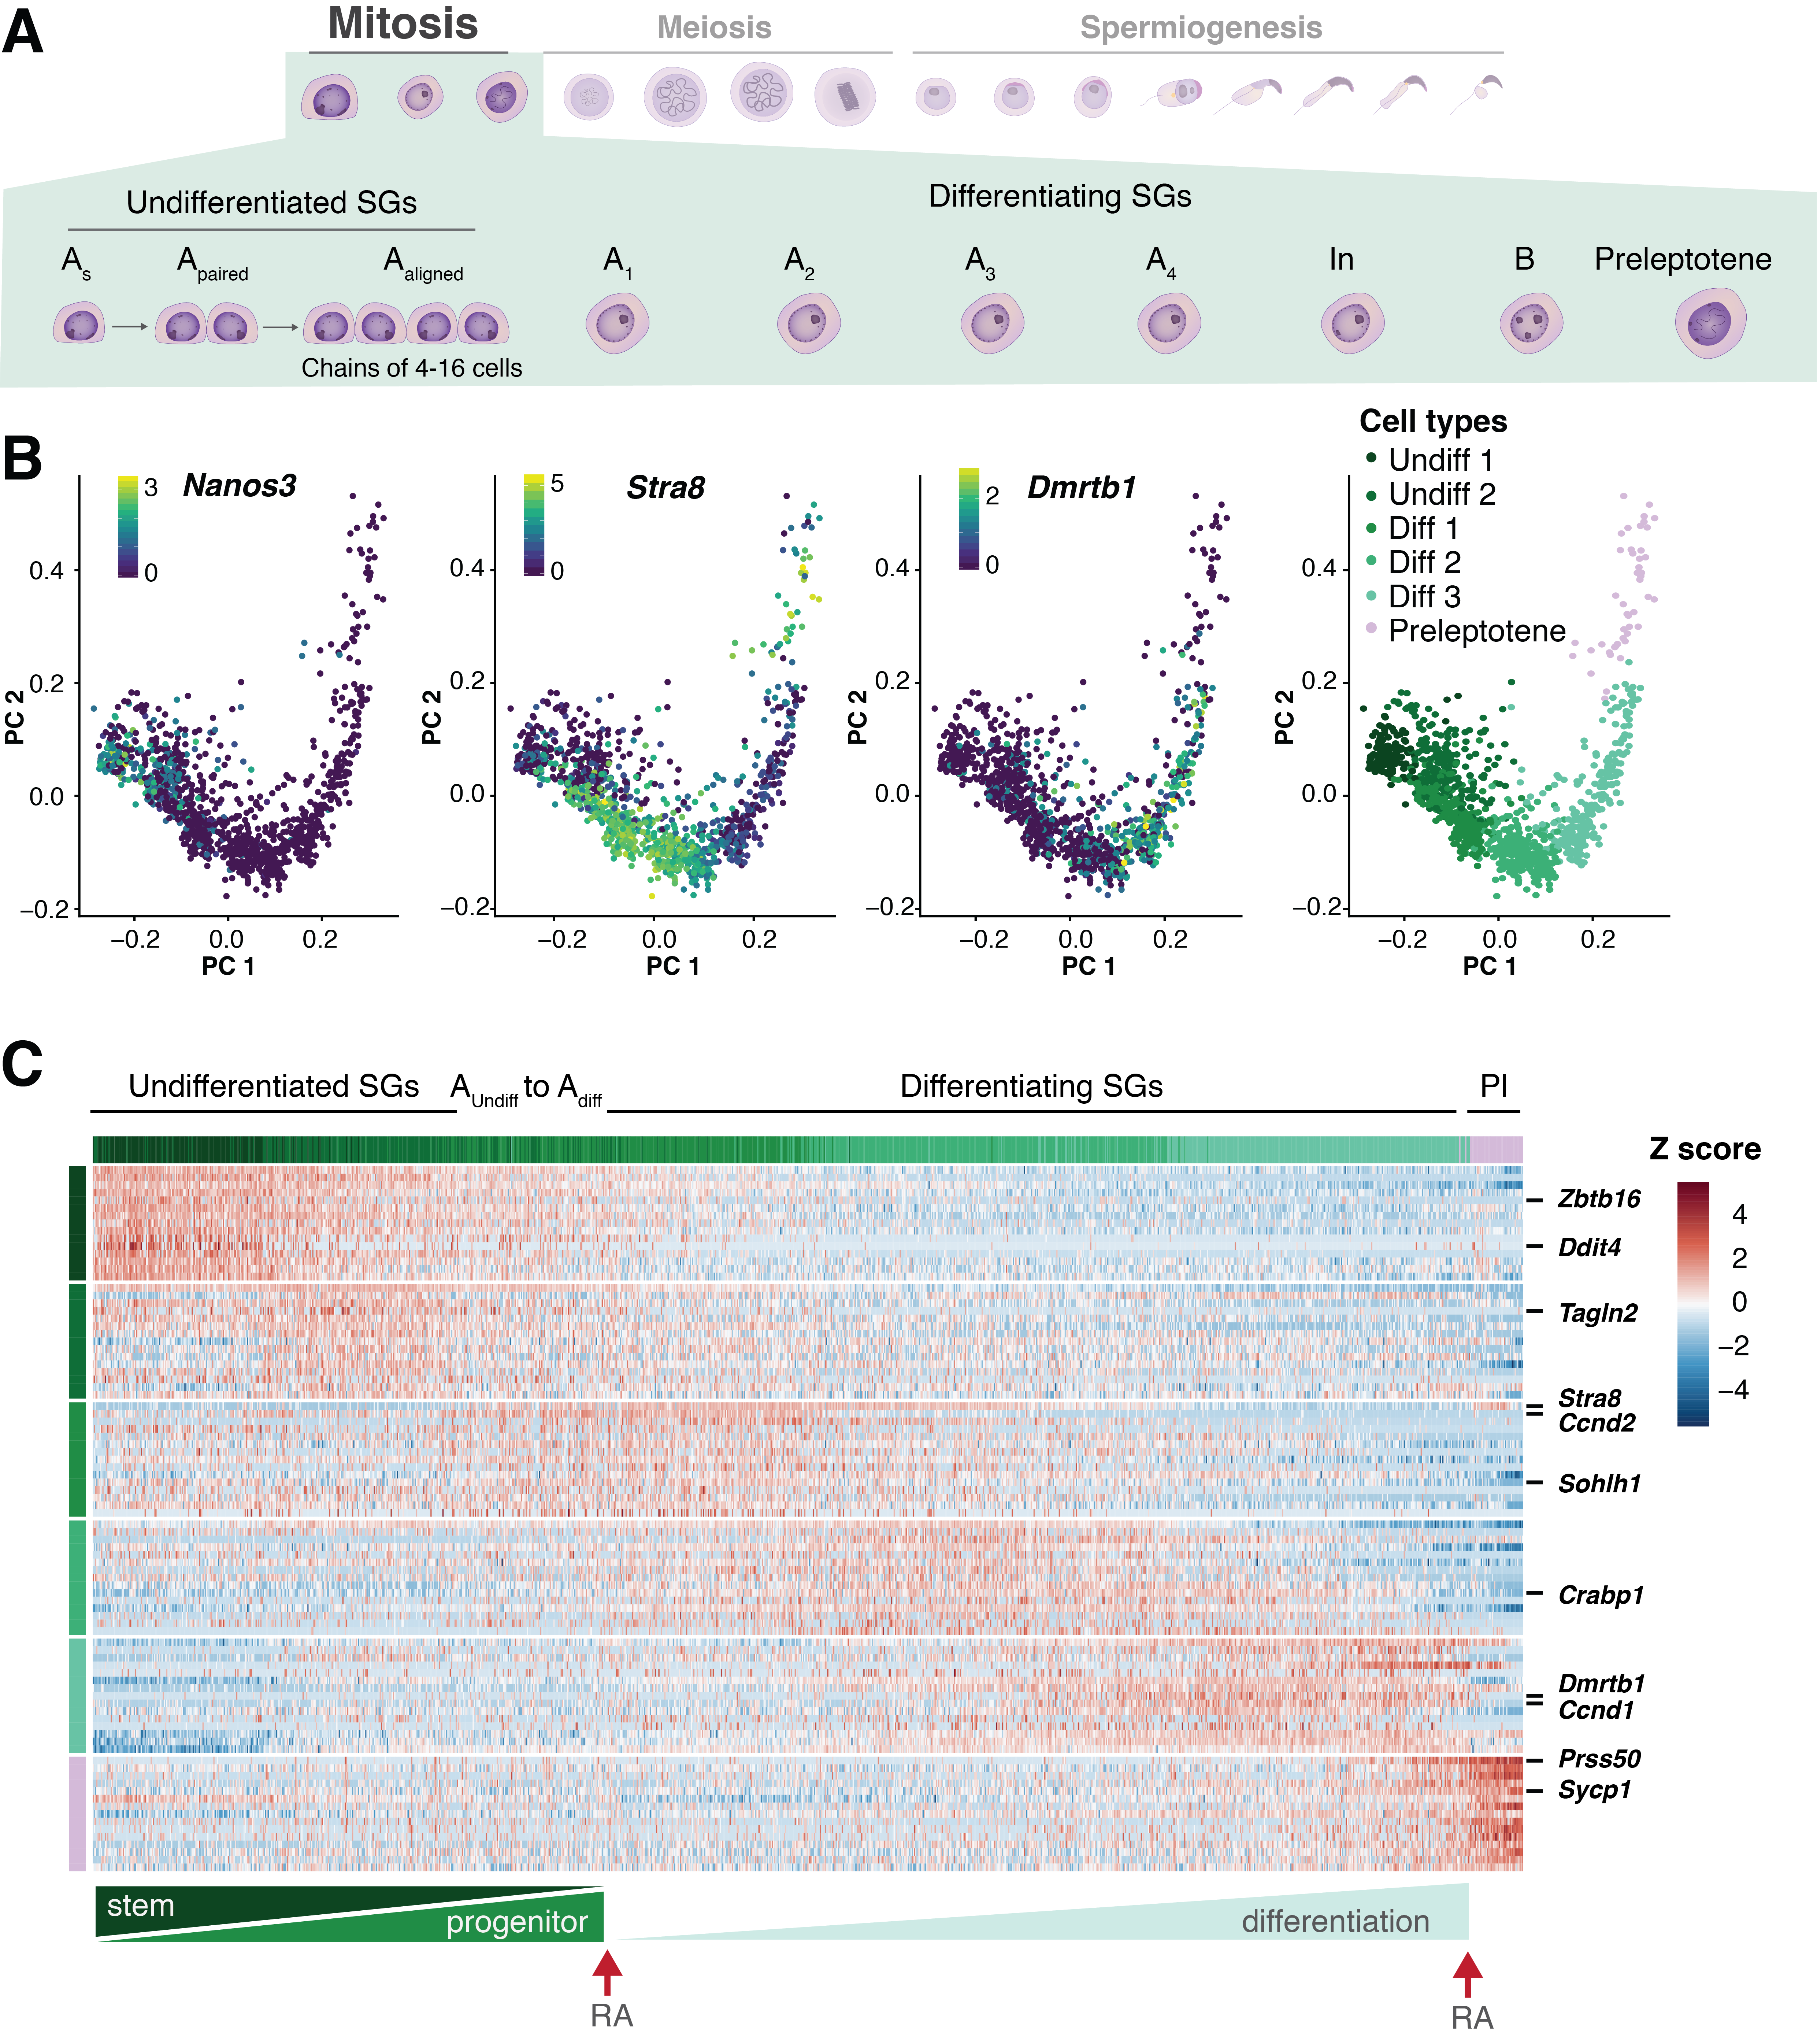
\includegraphics[width=\textwidth]{Fig_6.png}
\caption[DNA, epigenetic and translational features that modulate expression noise]{\textbf{DNA, epigenetic and translational features that modulate expression noise.}\\
Promoter sequence, number of transcription factor (TF) binding sites (TFBS, number of transcriptional start sites (TSS), enhance elements, RNA polymerase II (RNAPII) loading, DNA methylation, nucleosome positioning, histone modifications, polycomb repressive complex binding, miRNAs, nuclear export of mRNA, ribosome binding and blockage via stem loop formation are features that induce gene-specific intrinsic noise.}
\label{fig0:overview_intrinsic}
\end{figure}

\subsubsection{DNA features}

One of the key regulatory steps prior to RNA synthesis is the binding of \glspl{TF} to specific DNA sequences within the regulatory region of a gene which then triggers the controlled production of primary RNA transcripts from the DNA of this gene \citep{Latchman1993}. Mutations in the DNA sequence such as \glspl{SNV} can alter the binding affinity of TFs and therefore the rate at which a gene is expressed \textbf{(Fig.~\ref{fig0:DNA_features})}. A systematic study of the \textit{\gls{TDH3}} gene expression in yeast found that mutations in known \glspl{TFBS} decrease mean expression and increase expression noise. Moreover, Metzger \textit{et al.}, 2015 showed that evolutionary selection removes mutations that increase expression noise and that SNVs with large effects on expression noise show the lowest frequency within samples yeast strains \citep{Metzger2015}. \\

One of the most widely studied DNA motifs in relation to transcriptional noise is the TATA-box motif in promoters. Generally, TATA-box containing promoters show high levels of transcriptional noise \textbf{(Fig.~\ref{fig0:DNA_features})} \citep{Faure2017} possibly due to a simple activation cycle containing one or few inactive states \citep{Zoller2015}. Stress response genes are enriched for the TATA-box motif and allow an early adjustment to changing environmental conditions \citep{Lopez-Maury2009}. Moreover, TATA-box containing genes show an increased interspecies variability \citep{Tirosh2006} and higher spontaneous mutational variation \citep{Landry2007} indicating an increased evolvability of these particular genes. In an early study, Raser \textit{et al.}, 2004 studied the noisy expression controlled by the budding yeast \textit{\gls{PHO5}} promoter. This promoter contains the TATA-box motif and is has been shown that transcriptional noise is reduced when a mutational modification decreases the TATA-box strength \citep{Raser2004}. A more recent study confirmed this result and found mutations in yeast promoters that eliminate the TATA-box motif which resulted in reduced noise levels for these genes \citep{Hornung2012}. \\

A possible confounding factor for the increased noise of TATA-box containing promoters is the number of TFBSs. Tirosh \textit{et al.}, 2006 detected a two-fold enrichment of TBFSs in TATA-box containing promoters \citep{Tirosh2006}. A later study showed that transcriptional noise scales with increased numbers of TFBSs \textbf{(Fig.~\ref{fig0:DNA_features})} \citep{Sharon2014}. Furthermore, TATA-box containing genes lack enhancing histone marks and their increased variability in expression can therefore be explained by repressed chromatin \citep{Choi2008} (see \textbf{Section \ref{sec0:epigenetic}} ).  \\

Promoters can be classified based on their shape as narrow with few \glspl{TSS} that predominantly control tissue-specific gene expression and broad promoters with larger numbers of TSSs that control the expression of house keeping genes. Mutations that alter the shape of promoters increase transcriptional noise \citep{Schor2017a}. Furthermore, promoters with one or few TSS show higher levels of expression variability \textbf{(Fig.~\ref{fig0:DNA_features})} \citep{Faure2017}.\\

In addition to SNVs, \glspl{CNV} (usually defined as copy number variability of regions $\geq$ 1kb in comparison to a reference genome) in parts of the genome influence gene expression and contribute to, for example, schizophrenia and autism \citep{Gamazon2015}. Combined analysis of DNA and RNA has shown that genes with low copy number tend to be noisier expressed compared to genes with multiple copies \textbf{(Fig.~\ref{fig0:DNA_features})} \citep{Dey2015}. In the context of monoallelic expression, genes located on the X chromosome show increased mRNA half-life which in turn increases transcript stability reduces noise  to levels of autosomal genes \citep{Faure2017}.

\begin{figure}[!h]
\centering
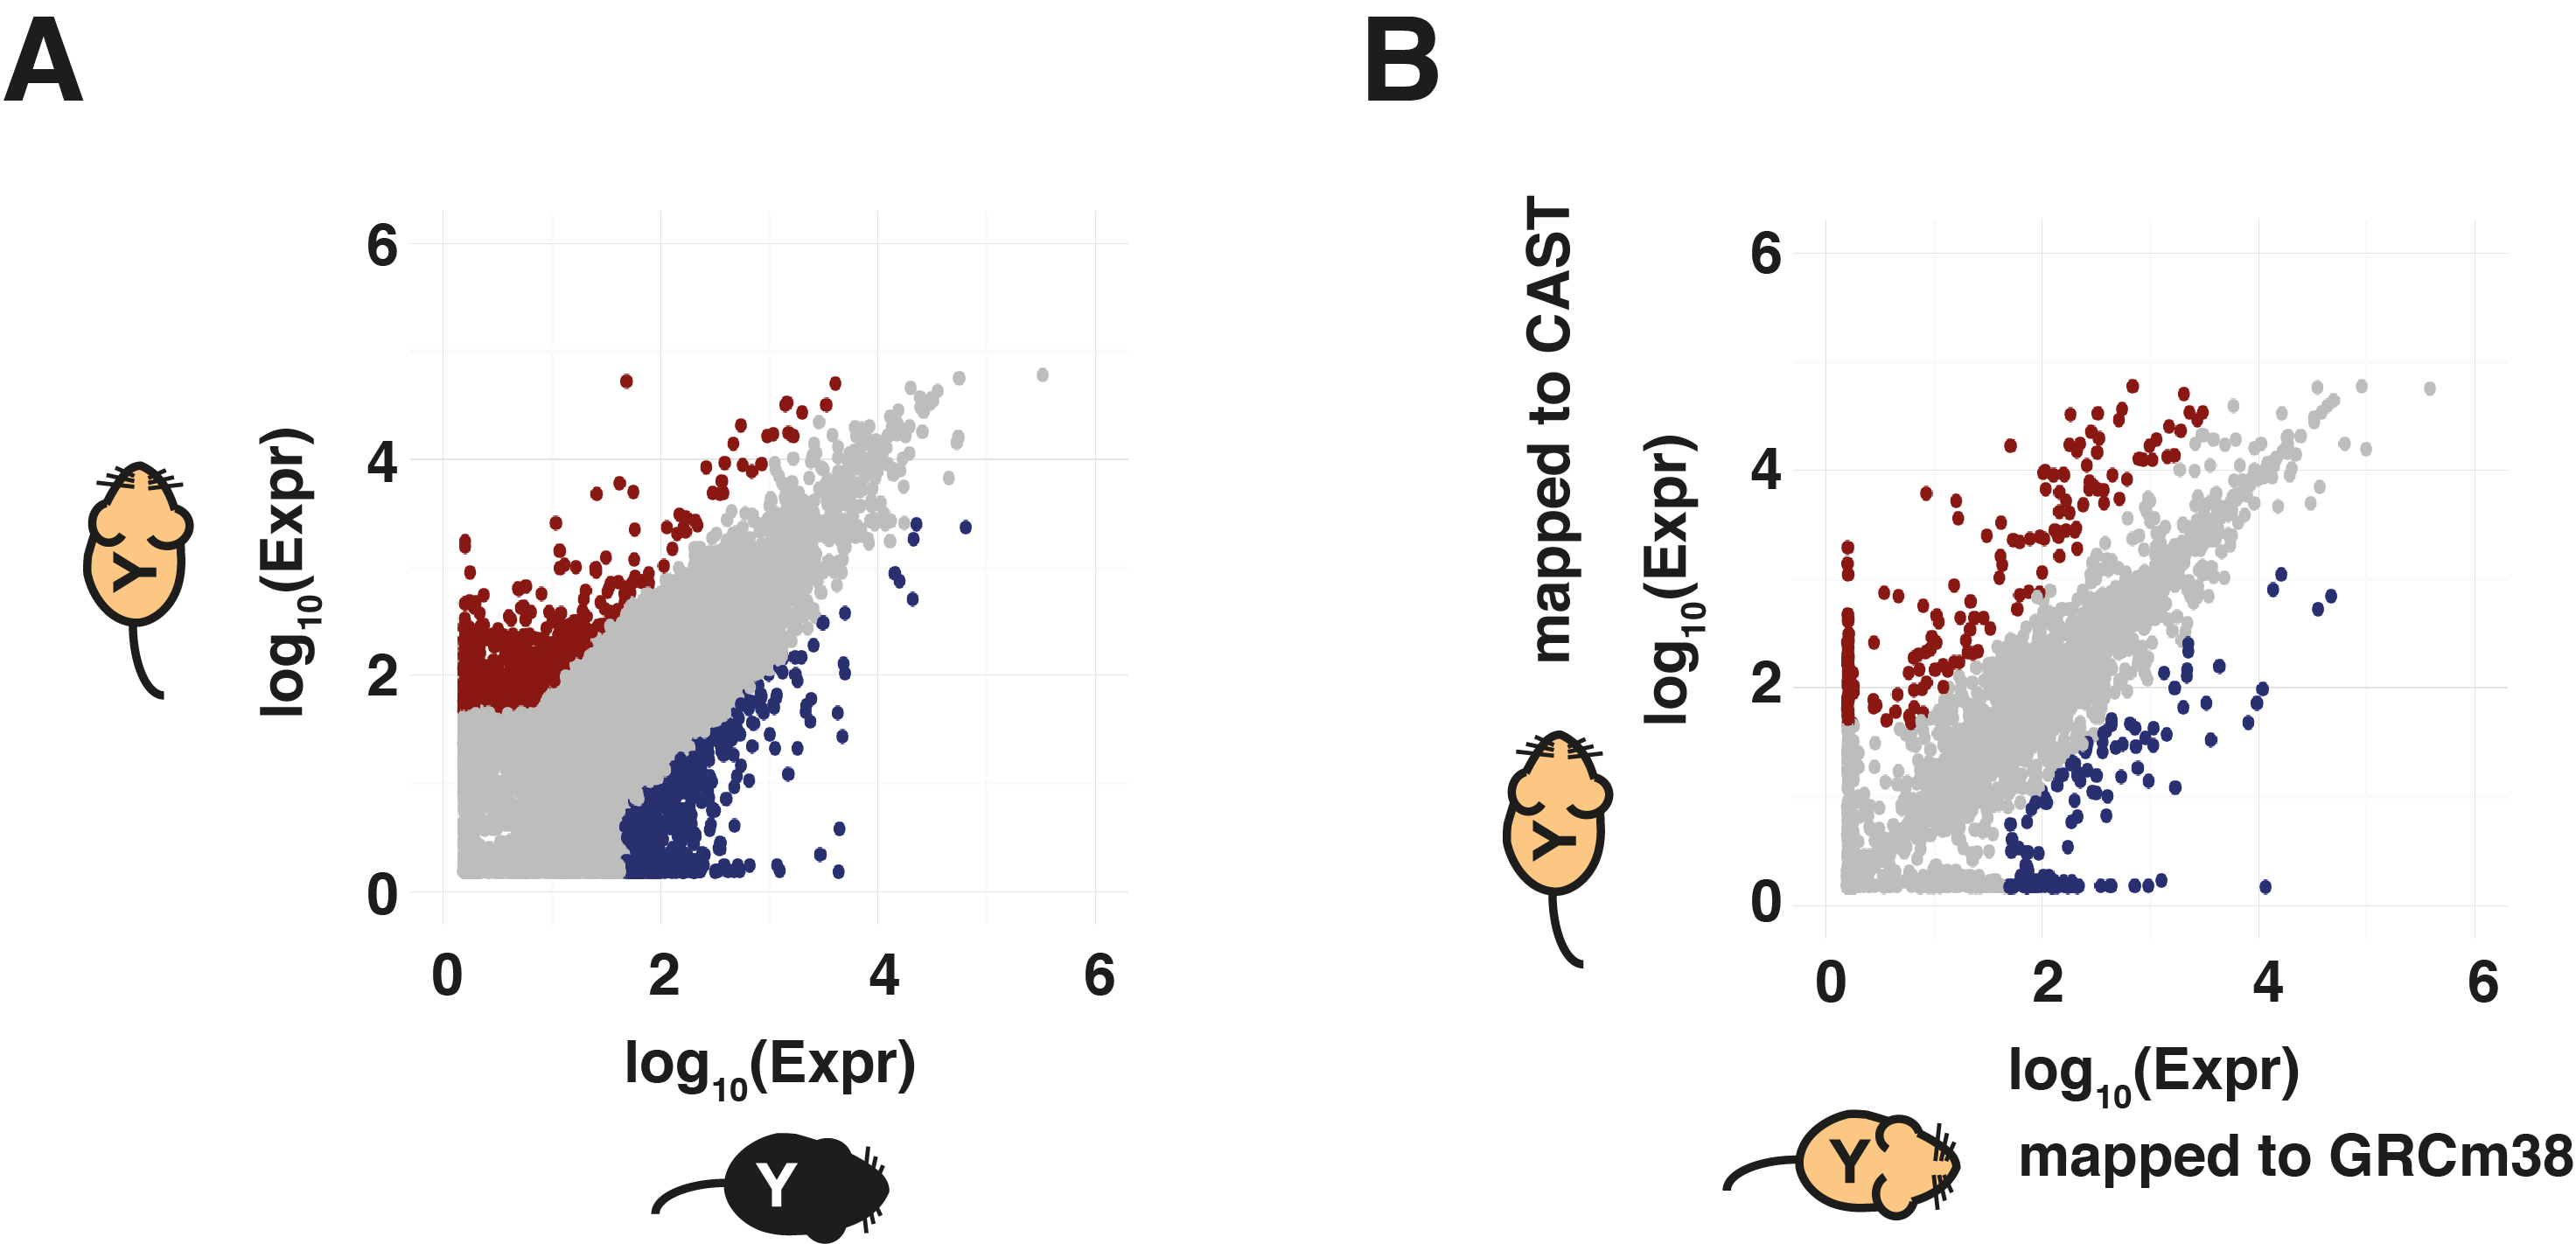
\includegraphics[width=0.85\textwidth]{Fig_7.png}
\caption[Features of the DNA sequence induce expression noise]{\textbf{Features of the DNA sequence induce expression noise.}\\
Mutations of the transcription factor (TF) binding site (TFBS), the presence of a TATA box, increase number of TFBSs, reduced number of transcriptional start sites (TSS) and reduced copy number of genes can induce transcriptional noise.}
\label{fig0:DNA_features}
\end{figure}

\subsubsection{Epigenetic factors}
\label{sec0:epigenetic}

Epigenetic factors are generally described as DNA methylation at \gls{CpG} dinucleotides, histone modifications and nucleosome positioning  \citep{Portela2010} and is defined as "the study of changes in gene function that are mitotically and/or meiotically heritable and that do not entail a change in DNA sequence" \citep{Wu2001}. \\

CpG islands are genomic sites of more than 200 bases with a GC content of more than 50\% where DNA methylation can preferentially occur. Methylation of CpG islands in promoters represses transcription while methylation in gene bodies facilitates transcription \citep{Portela2010}.  Recently, the presence of CpG islands in gene bodies but also at the TSS and in promoter regions was linked to a reduction in transcriptional noise \citep{Faure2017}. Similarly, previous findings showed that expression noise scales negatively with gene body methylation \cite{Huh2013}. Morgan and Marioni, 2018 studied the effect of CpG island size on transcriptional noise using scRNA-Seq data. Genes associated with short CpG island promoters tend to be noisier expressed than genes with long CpG island promoters. Furthermore, early response genes during \gls{LPS} stimulation of bone-marrow derived dendritic cells and heregulin stimulation of human breast cancer cells are enriched for those with short CpG island promoters \citep{Morgan2018}. \\

Modifications of histones induce the activation or repression of chromatin and  therefore indirectly modulate gene expression\citep{Suganuma2011}. In an extensive study to link histone modifications to transcriptional noise, Faure \textit{et al.}, 2017 detected several histone modifications in promoter/core promoter motifs, at the TSS and in gene bodies to increase or decrease noise. The repressive \gls{H3K27me3} mark is linked to higher noise levels when present at the TSS, in promoters and in gene bodies. The enhancer related \gls{H3K4me1} mark only increases noise when present at the TSS and in the core promoter sequence while the repressive \gls{H3K9me3} mark increases noise when present in the promoter motif. The activating marks \Gls{H3K4me3}, \gls{H3K9ac} and \gls{H3K36me3} are linked to low levels of noise when present in gene bodies. In addition to these single features, bivalent promoters that carry the repressive \gls{H3K27me3} and enhancing \gls{H3K4me3} marks show high levels of transcriptional noise \citep{Faure2017}.\\ 

Polycomp repressive complexes (PRCs) are epigenetic modifiers of histones to repress transcription of developmental genes \citep{Chittock2017}. They can bind together with active \gls{RNAPII} to bivalent promoters and switching between the repressed and active states introduces gene expression variability across a population of cells \cite{Kar2017}. Additionally, deletions of different histone deacetylation complexes (Set3C and Rpd3(L)), that both repressed transcription by removing H3K9ac, showed different effects on transcriptional bursting \citep{Weinberger2012}.  Confirming this, a later study showed that gene body and promoter histone modifications independently influence burst size and burst frequency and therefore regulate mean expression and noise in an uncoupled fashion \cite{Wu2017}. These results indicate a fine-tuned regulation of transcriptional noise and support the functional role of biological noise in cell populations.\\

Chromatin is the packaged state of DNA within the nucleus and its central element are nucleosomes. Nucleosomes are made up of eight of the four histones (H3, H4, H2A, H2B) and 147 bases of DNA can wrap around this complex. An array of histone modifying enzymes exits that regulate the opening or closing of the chromatin; termed heterochromatin and euchromatin respectively \citep{Kouzarides2007}. Tirosh \textit{et al.}, 2008 showed that promoters with high nucleosome occupancy close to the TSS tend to display a high range of expression levels across varying conditions (transcriptional plasticity). Distant nucleosome-rich regions are on the other hand associated with low transcriptional noise \citep{Tirosh2008}. Nucleosome covered promoters display shorter transcriptional rates, which in turn explains increased transcriptional noise for these promoters \cite{Dey2015}. Single-cell measures indicate cell-to-cell variations in nucleosome positioning around the \textit{PHO5} promoter upon stress induction. Even in the non-stressed state, a small fraction of cells exhibit nucleosome free regions at the promoter which explains low and possibly noisy expression of \textit{PHO5} \citep{Small2014}. Deletion of chromatin remodeling complexes that remove nucleosomes upon transcription factor binding results in increased transcriptional noise compared to wild-type cells \citep{Raser2004}. \\ 

Boundaries between heterochromatin and euchromatin are controlled by boundary elements, such as the transcription factor \Gls{CTCF}, that recruit chromatin modifying factors \citep{Kouzarides2007}. CTCF also regulates transcription by activating or repressing promoters and regulates distant chromatin interactions \citep{Kim2015a}. Recent studies suggest that long-range enhancer-promoter interactions modulate transcriptional noise. Interference of CTCF-mediated enhancer-promoter contact either by CTCF knock-out or CTCF-binding site deletion leads to increased expression variability in selected genes \citep{Ren2017}. Enhancers are cis-regulatory elements, non-coding DNA with TFBSs, that regulate the expression of neighbouring genes \citep{Blackwood1998}. Genes within super-enhancer loci, a region with multiple enhancers, controlling pluripotency master regulators show high levels of variability in expression and down-stream targets of these master regulators show similar co-variation across mESCs \citep{Faure2017}.\\

Moreover, the positioning of genes on the genome controls expression noise with densely clustered genes being less noisy expressed in comparison to non-clustered genes \citep{Kustatscher2017}. Additionally, genes positioned next to “noisy” genes display higher levels of transcriptional variability compared to genes that are located in proximity to “stable” genes \citep{Kar2017}. Expression noise is also increased for genes that are located in a repressed neighborhood, namely active genes in constitutive nuclear lamina-associated domains \citep{Faure2017}.\\

\textbf{Table \ref{tab0:epigenetic}} summarises the relation between epigenetic features and noisy gene expression.

\begin{table}[hb	]
\centering
\caption{Epigenetic control of transcriptional noise}
\label{tab0:epigenetic}
\begin{tabular}{l l c c}
\toprule
\toprule
 & Feature & Noisy & Stable \\ 
\midrule
\midrule
\multirow{3}{*}[-2pt]{DNA methylation} & CpG islands &  & \checkmark{} \\
\cmidrule{2-4}
& Short CpG islands & \checkmark{} &  \\
\cmidrule{2-4}
& Gene body methylation &  & \checkmark{} \\
\midrule
\multirow{7}{*}[-2pt]{Histone modification} & H3K27me3 (TSS, promoter, gene body) & \checkmark{}  & \\
\cmidrule{2-4}
& H3K4me1 (TSS, promoter) & \checkmark{}  & \\
\cmidrule{2-4}
& H3K9me3 (promoter) & \checkmark{}  & \\
\cmidrule{2-4}
& H3K4me3 (gene bodies) &  & \checkmark{}\\
\cmidrule{2-4}
& H3K9ac (gene bodies) &  & \checkmark{} \\
\cmidrule{2-4}
& H3K36me3 (gene bodies) &  & \checkmark{} \\
\cmidrule{2-4}
& H3K27me3 and H3K4me3 & \checkmark{}  & \\
\midrule
\multirow{3}{*}[-2pt]{Nucleosome position} & Nucleosome rich promoters & \checkmark{} & \\
\cmidrule{2-4}
& Distant nucleosome rich regions &  & \checkmark{} \\
\cmidrule{2-4}
& Deletion of nucleosome remodelling complexes & \checkmark{}  & \\
\midrule
\multirow{7}{*}[-2pt]{Genome architecture} & CTCF knock-out & \checkmark{} & \\
\cmidrule{2-4}
& CTCF binding site depletion & \checkmark{} & \\
\cmidrule{2-4}
& Clustered genes &  & \checkmark{} \\
\cmidrule{2-4}
& Nuclear-lamina associated genes & \checkmark{} & \\
\bottomrule
\bottomrule
\end{tabular}
\end{table} 

\newpage

\subsubsection{Transcriptional features}

Transcription is initiated by TFs binding to specific regulatory DNA sequences followed by recruitment of RNAPII, RNA synthesis and RNA degradation. As discussed above, promoter architecture, namely the location and accessibility of TFBS and RNAPII binding sites, dictates mean expression and transcriptional noise. \\

In bacteria, the intracellular physical distance between TF source and the promoter sequence influences expression variability. TF expression proximal to their target genes results in less noisy expression compared to regulator sources distant to the promoter sequence \citep{Goni-Moreno2017}. Once TFs bind to their target sequence, Carey \emph{et al.}, 2013 showed that mean expression to noise ratio is promoter dependent while in the majority of cases, noise negatively scales with mean expression \citep{Carey2013}. \\

Similar to TF binding dynamics, the assembly of RNAPII complexes modulates transcriptional noise. An early study identified the connection between paused RNAPII and synchronous expression of target genes. Genes without pre-loaded RNAPII show more stochastic activation patterns \citep{Boettiger2009}. This finding has later been confirmed using scRNA-Seq data while increased variability was detected for genes with non-pause RNAPII across the full range of expression levels \citep{Day2016}.\\

\begin{figure}[!h]
\centering
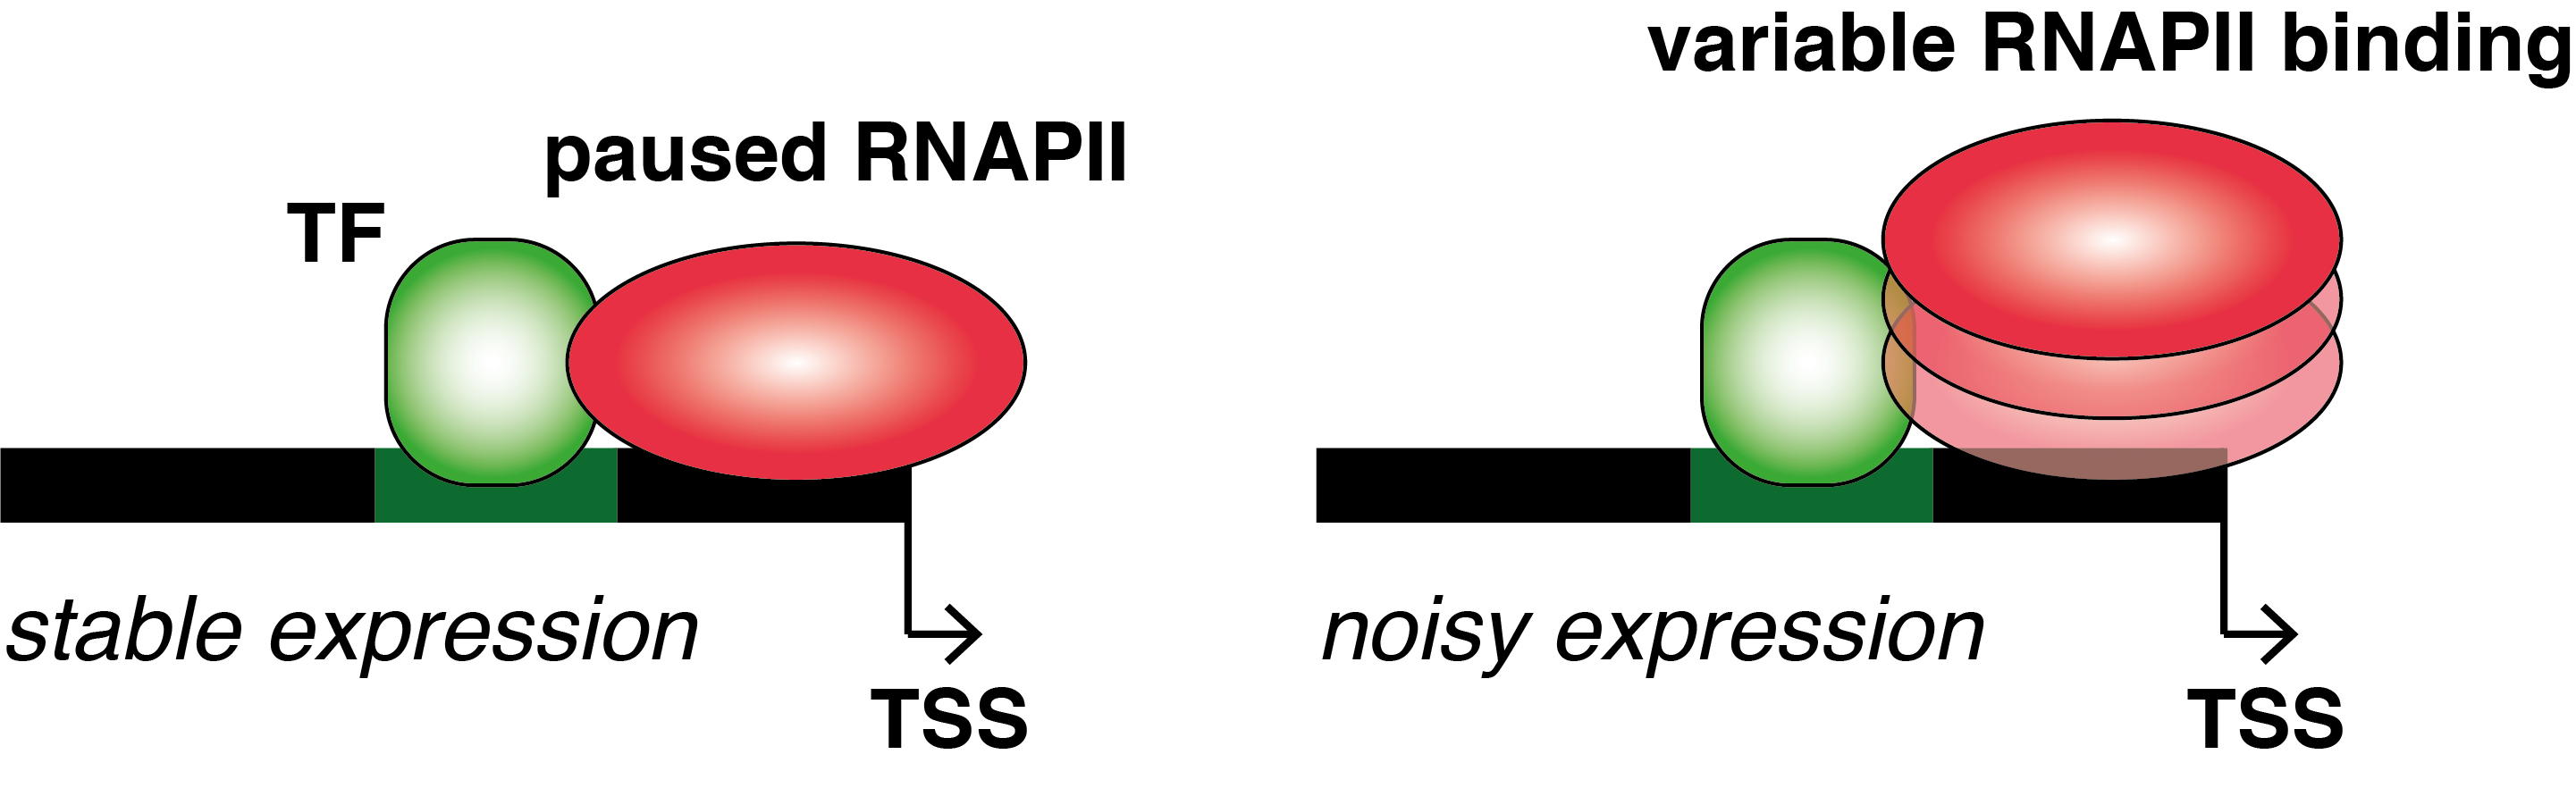
\includegraphics[width=0.7\textwidth]{Fig_8.png}
\caption[RNAPII pausing reduces transcriptional noise]{\textbf{RNAPII pausing reduces transcriptional noise.}\\
Left: Pre-loaded RNA polymerase II (RNAPII) allows direct transcription upon transcription factor (TF) binding. Right: RNAPII recruitment induces gene expression variability.}
\label{fig0:DNA_features}
\end{figure} 

\newpage

\subsubsection{Post-transcriptional and translational features}

After synthesis, pre-RNAs are polyadenylated and spliced to form mRNA that relocates from the nucleus to the cytoplasm where translation occurs to synthesise proteins \cite{Glisovic2008}. On the post-transcriptional and translational level, mRNA localization, structure, degradation and translation have been shown to influence cell-to-cell variations in protein abundance.

Upon transcriptional activation, RNAs are produced in burst-like patterns while burst frequency modulates mean expression and noise, and burst size influences solely mean expression \citep{Hornung2012}. While bursty transcript synthesis introduces stochastic fluctuations in nuclei between cells, active export of mRNAs into the cytoplasm can dampen this source of variability \citep{Battich2015a}. Reduces cytoplasmatic noise has also been shown for two nuclearly retained genes in the mammalian liver. Furthermore, this mode of noise control was proposed to be active across a range of metabolic tissues \cite{BaharHalpern2015a}.\\

\begin{figure}[!h]
\centering
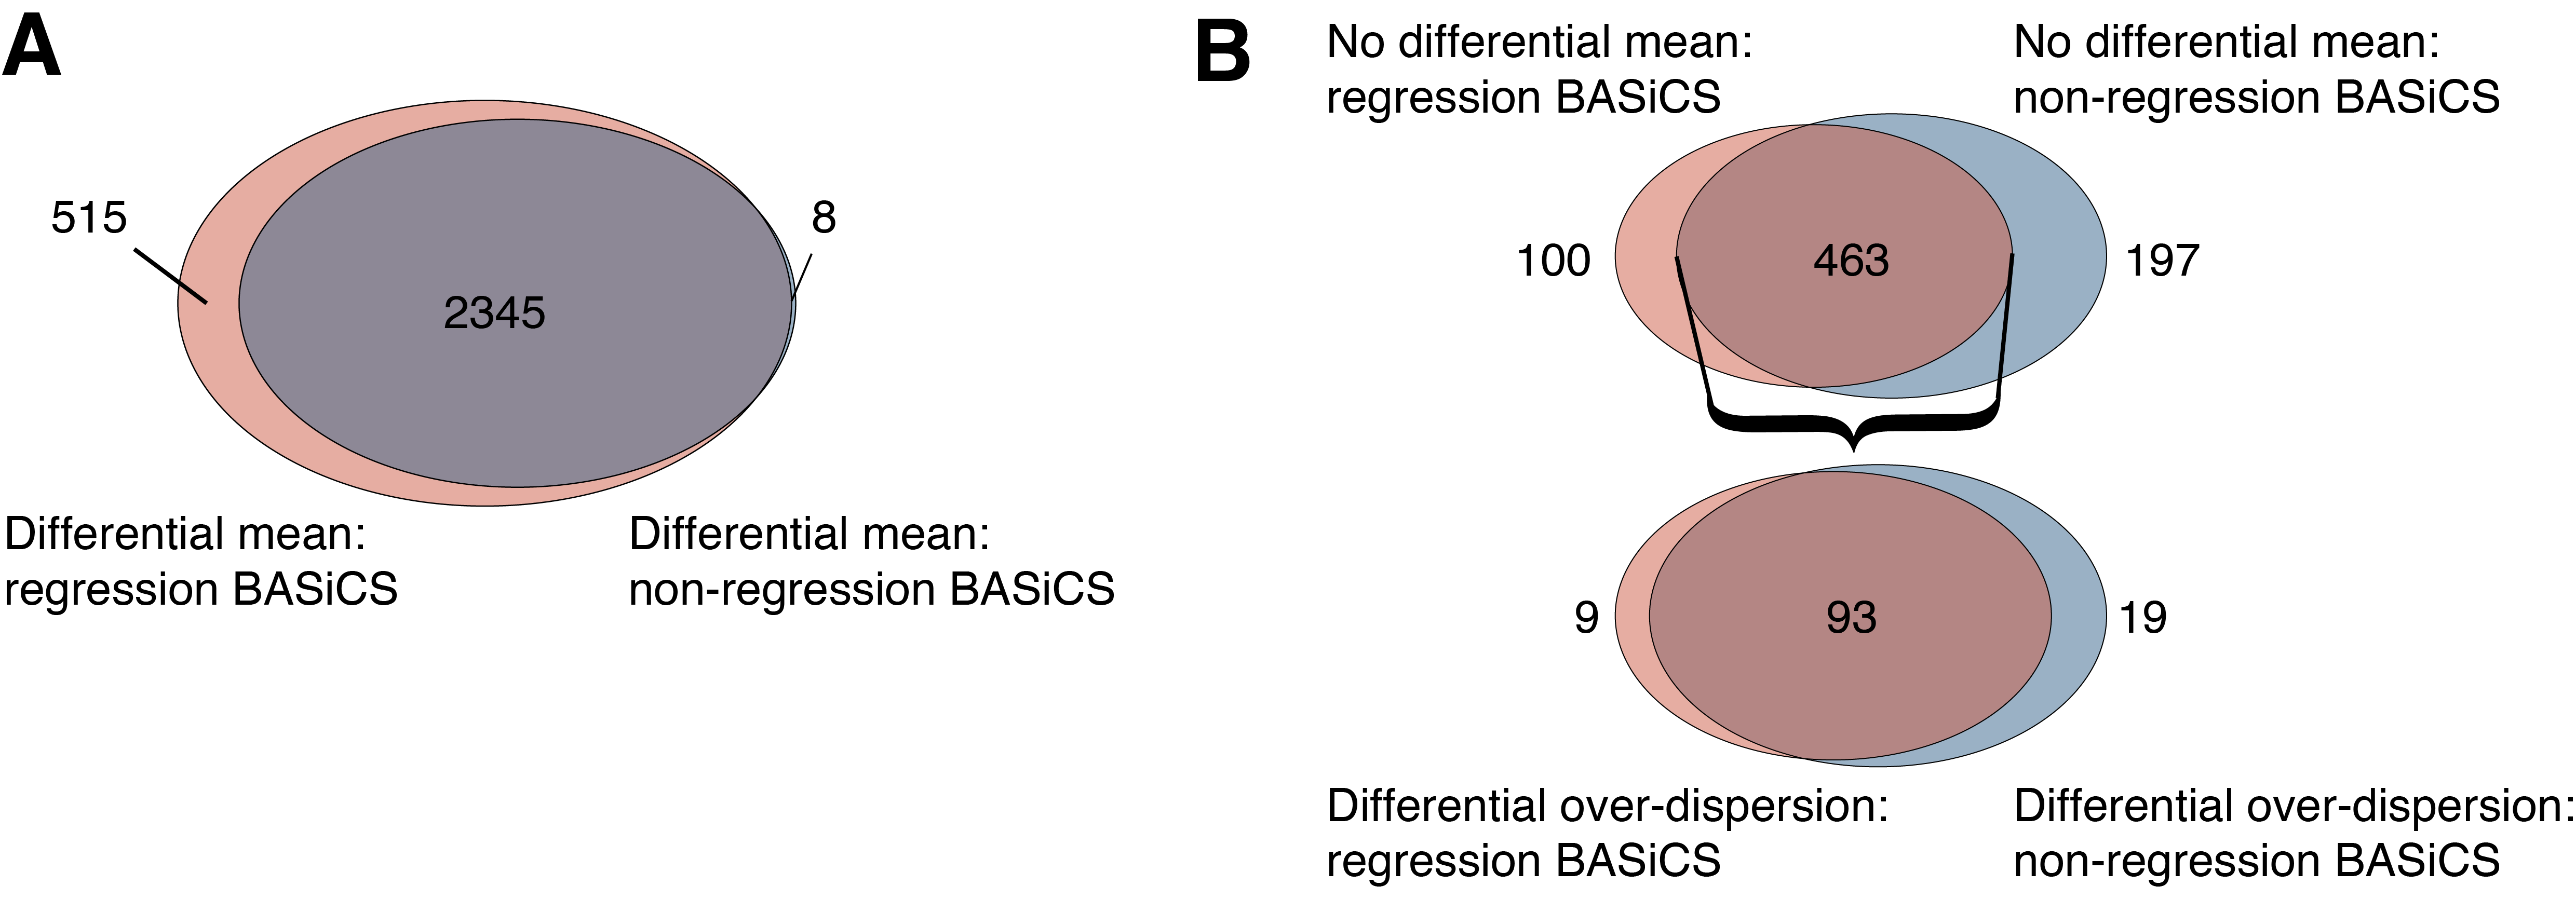
\includegraphics[width=\textwidth]{Fig_9.png}
\caption[Post-transcriptional regulation to control noisy expression]{\textbf{Post-transcriptional regulation to control noisy expression.}\\
Bursty expression introduces nuclear variation in transcript abundance that is buffered due to retention at the nuclear membrane. Within the cytoplasm, micro RNAs degrade lowly expressed genes to reduce expression noise. Deletion of the ribsosome binding site as well as stem loop formation increase variability in protein abundance across cells. Arrows indicate either increased (red) or decreased noise (green) dependent on the regulatory mechanism.}
\label{fig0:DNA_features}
\end{figure} 

\newpage

Within the cytoplasm, mRNAs are subject to translation or degradation. At this stage, stochasticity from bursty gene expression is propagated to variation in protein abundance. The availability of mRNAs for translation is not only dictated by their syntheses but also their degradation rate. mRNA degradation is accelerated by recognition of micro RNAs. This process has been shown to preferentially reduce noise levels for lowly expressed genes in mESCs to possibly retain cellular identity \citep{Schmiedel2015}. Similarly, temporal averaging of long-lived transcripts reduces noise in mRNA abundance. In that way, increased transcript stability compensates for noise introduced by the single-allele expression of genes on chromosome X \citep{Faure2017}.  \\

In addition to noise introduced by stochastic processes on the transcriptional level, the recognition and binding of ribosomes to mRNAs for translation initiation features a source for variations in protein abundance. Modulating translational efficiency by mutating the ribosome binding site and initiation codon showed an interaction between translation and variation in protein abundance \citep{Ozbudak2002}. Additionally, mRNA secondary structure formed by stem loops and ploy(G) motifs affects translation initiation and increases noise in protein levels \citep{Dacheux2017a}.

\subsection{Extrinsic noise}

Extrinsic noise within a cell population arises from cells being in different regulatory states. Here, differences in cellular components introduce variation in mRNA and protein abundance. Examples for cell states in otherwise homogeneous populations are characterized by differences in metabolism, cell cycle, volume, cell-to-cell and environmental signalling as well as cell density. It has been shown that extrinsic noise forms a major contribution to variations in gene expression and that transcript distributions can be predicted from the cellular state, population context and microenvironment \citep{Battich2015a}.

\subsubsection{Cell cycle}

Cell cycle has been widely discussed to form a crucial source of extrinsic noise \citep{Colman-Lerner2005a, Newman2006}). In yeast populations, differences in transcriptional activities between the G1 and S/G2/M phases of the cell cycle lead to large-scale transcriptional heterogeneity across cell populations \citep{Zopf2013}. Under nutrient-poor conditions, growth rate is reduced and noise is elevated due to cells being in different cell-cycle stages \citep{Keren2015}.  Even under optimal growth conditions for mESCs (2i media), cell cycle related genes show strong heterogeneity in expression across the cell population \citep{Kolodziejczyk2015cell}. Nonetheless, sorting cells into similar cell cycle stages did not drastically reduce noise levels \citep{Raser2004}. When quantifying cell-to-cell variation, cell cycle induced extrinsic noise is often seen as unwanted variation and can mask more subtle transcriptional heterogeneity. Computational methods have been developed to correct for this confounding effect to enhance the underlying noise signal \citep{Buettner2015, Buettner2017}. 

\subsubsection{Cell volume}

Cellular volume provides another explanation for global differences in mRNA content between individual cells introducing large-scale transcriptional heterogeneity. Even though cell volume changes during cell cycle progression, within each phase cell volume varied as much as across all phases. It has been shown that mRNA counts scale with cellular volume to maintain transcript concentrations within each cell \citep{Kempe2015, Padovan-Merhar2015, Zhurinsky2010}. To avoid this source of heterogeneity, normalization approaches correct for differences in mRNA content between individual cells \citep{Vallejos2017}.

\subsubsection{Metabolism}

The effect of metabolic fluctuations has been studied in \textit{E. coli} populations. Variations in biochemical reactions are induced by noise in the expression of their corresponding catalytic enzymes. Changes in metabolism are then coupled to varying growth rates of individual cells, which in turn introduces large-scale transcriptional heterogeneity in cell populations \citep{Kiviet2014}.  

\subsubsection{Expression capacity}

Fluctuations in the expression capacity of cells due to quantitative differences in RNAPII or ribosomes induce global variability among the majority of proteins \citep{Colman-Lerner2005a}.

\subsubsection{Cell signalling}

A different source of extrinsic noise is the intra- or inter-cellular signalling state of individual cells. Fluctuations in membrane bound or cytoplasmic proteins lead to inconsistent transmission of signalling stimuli as exemplified by variability in TRAIL-induced apoptosis \citep{Spencer2009}. Similarly, variations of regulators in the \gls{ERK} signalling pathway introduce downstream variability in nuclear response. The degree of which nuclear ERK response is varied depends on the position of the regulator in the topology of the signalling pathway \citep{Iwamoto2016}. In \textit{C. elegans}, perturbation of the Wnt signalling pathway displayed different degrees of variability in expression of the key Hox gene for Q neuroblast migration, \textit{mab-5}. It has been proposed that extrinsic noise, in this case the strength of the Wnt signal, modulates intrinsic variation in the expression of \textit{mab-5} \citep{Ji2013}. 

\subsubsection{Physical constrains}

Physical constrains on cell growth and the direct population context influence the state of individual cells \citep{Battich2015a}. Snijder \textit{et al.}, 2009 performed detailed imaging based analysis of adherent human cells that were infected with different viruses. Clathrin mediated endocytosis was most variable with low cell density leading to inefficient mouse hepatits virus infection. Dengue virus preferentially infects edge cells while simian virus 40 infection was decreased with large cell density \citep{Snijder2009}. These experiments indicate the importance of local cellular microenvironment and cell-cell contacts leading to heterogeneity in cell states. 


\newpage
%!TEX root = ../intro.tex
%******************************
%	 Quantification of biological noise
%*****************************

\section{Quantification of cell population heterogeneity} 

To quantify biological noise in cellular systems, single-cell approaches employ either sequencing or imaging technologies to extract genomic, transcriptomic, epigenetic or proteomic features from individual cells. These technologies show specific advantages and limitations on the level of throughput and content. 
In this section, I will discuss the applicability of single-cell sequencing and imaging technologies as a potential read-out for cell population heterogeneity induced by transcriptional noise.

\subsection{Single-cell sequencing}

Next generation sequencing approaches have been applied to individual cells to quantify variation in DNA sequence, mRNA expression, epigenetic marks and protein abundance within a cell population. 

\subsubsection{Single-cell whole genome sequencing}

\Gls{scDNA-Seq} has previously been used to identify CNVs and SNVs between single cells \citep{Zong2012}. 
Based on these read-outs, tumour heterogeneity and evolution \citep{Navin2011} as well as lineage relationships in the human brain were inferred \citep{Evrony2015}. 
To obtain enough genomic material, \gls{WGA} is performed on DNA from individual cells. The \gls{SCOMP} degrades DNA via restriction enzymes, includes a primary \gls{PCR} amplification step and a later re-amplification via comparative genomic hybridisation \citep{Klein1999}. \Gls{MDA} is based on the random initiation of amplification via oligonucleotide primers with strand displacement \citep{Dean2002}. Compared to MDA, \gls{MALBAC} achieves an initial quasi-linear amplification step by pre-amplification using primers with handle sequences. 
Full amplicons form hairpins that are exponentially amplified prior to sequencing \citep{Zong2012}. \\

The main limitation of single-cell DNA sequencing is the genomic coverage per cell. 
While the detection of SNVs requires deep sequencing of individual cells, CNVs can be detected with shallow sequencing therefore allowing the throughput to increase \textbf{(Fig.~\ref{fig0:scDNA-Seq})} \citep{Knouse2016, Baslan2015}. 
Recently, Vitak \emph{et al.}, 2017 introduced \gls{sci-Seq} which allows the generation of thousands of single-cell genomes for sequencing. 
In the first step, multiple nuclei are sorted into each well of a 96 well plate and the genomic DNA is labelled with barcodes by transposase tagging. 
In the second step, 15-25 tagged cells are sorted into individual wells of a PCR plate where the second round of barcoding is performed during amplification. In that way, CNVs of over 15,000 cells can be assessed \citep{Vitak2017}.

\begin{figure}[!h]
\centering
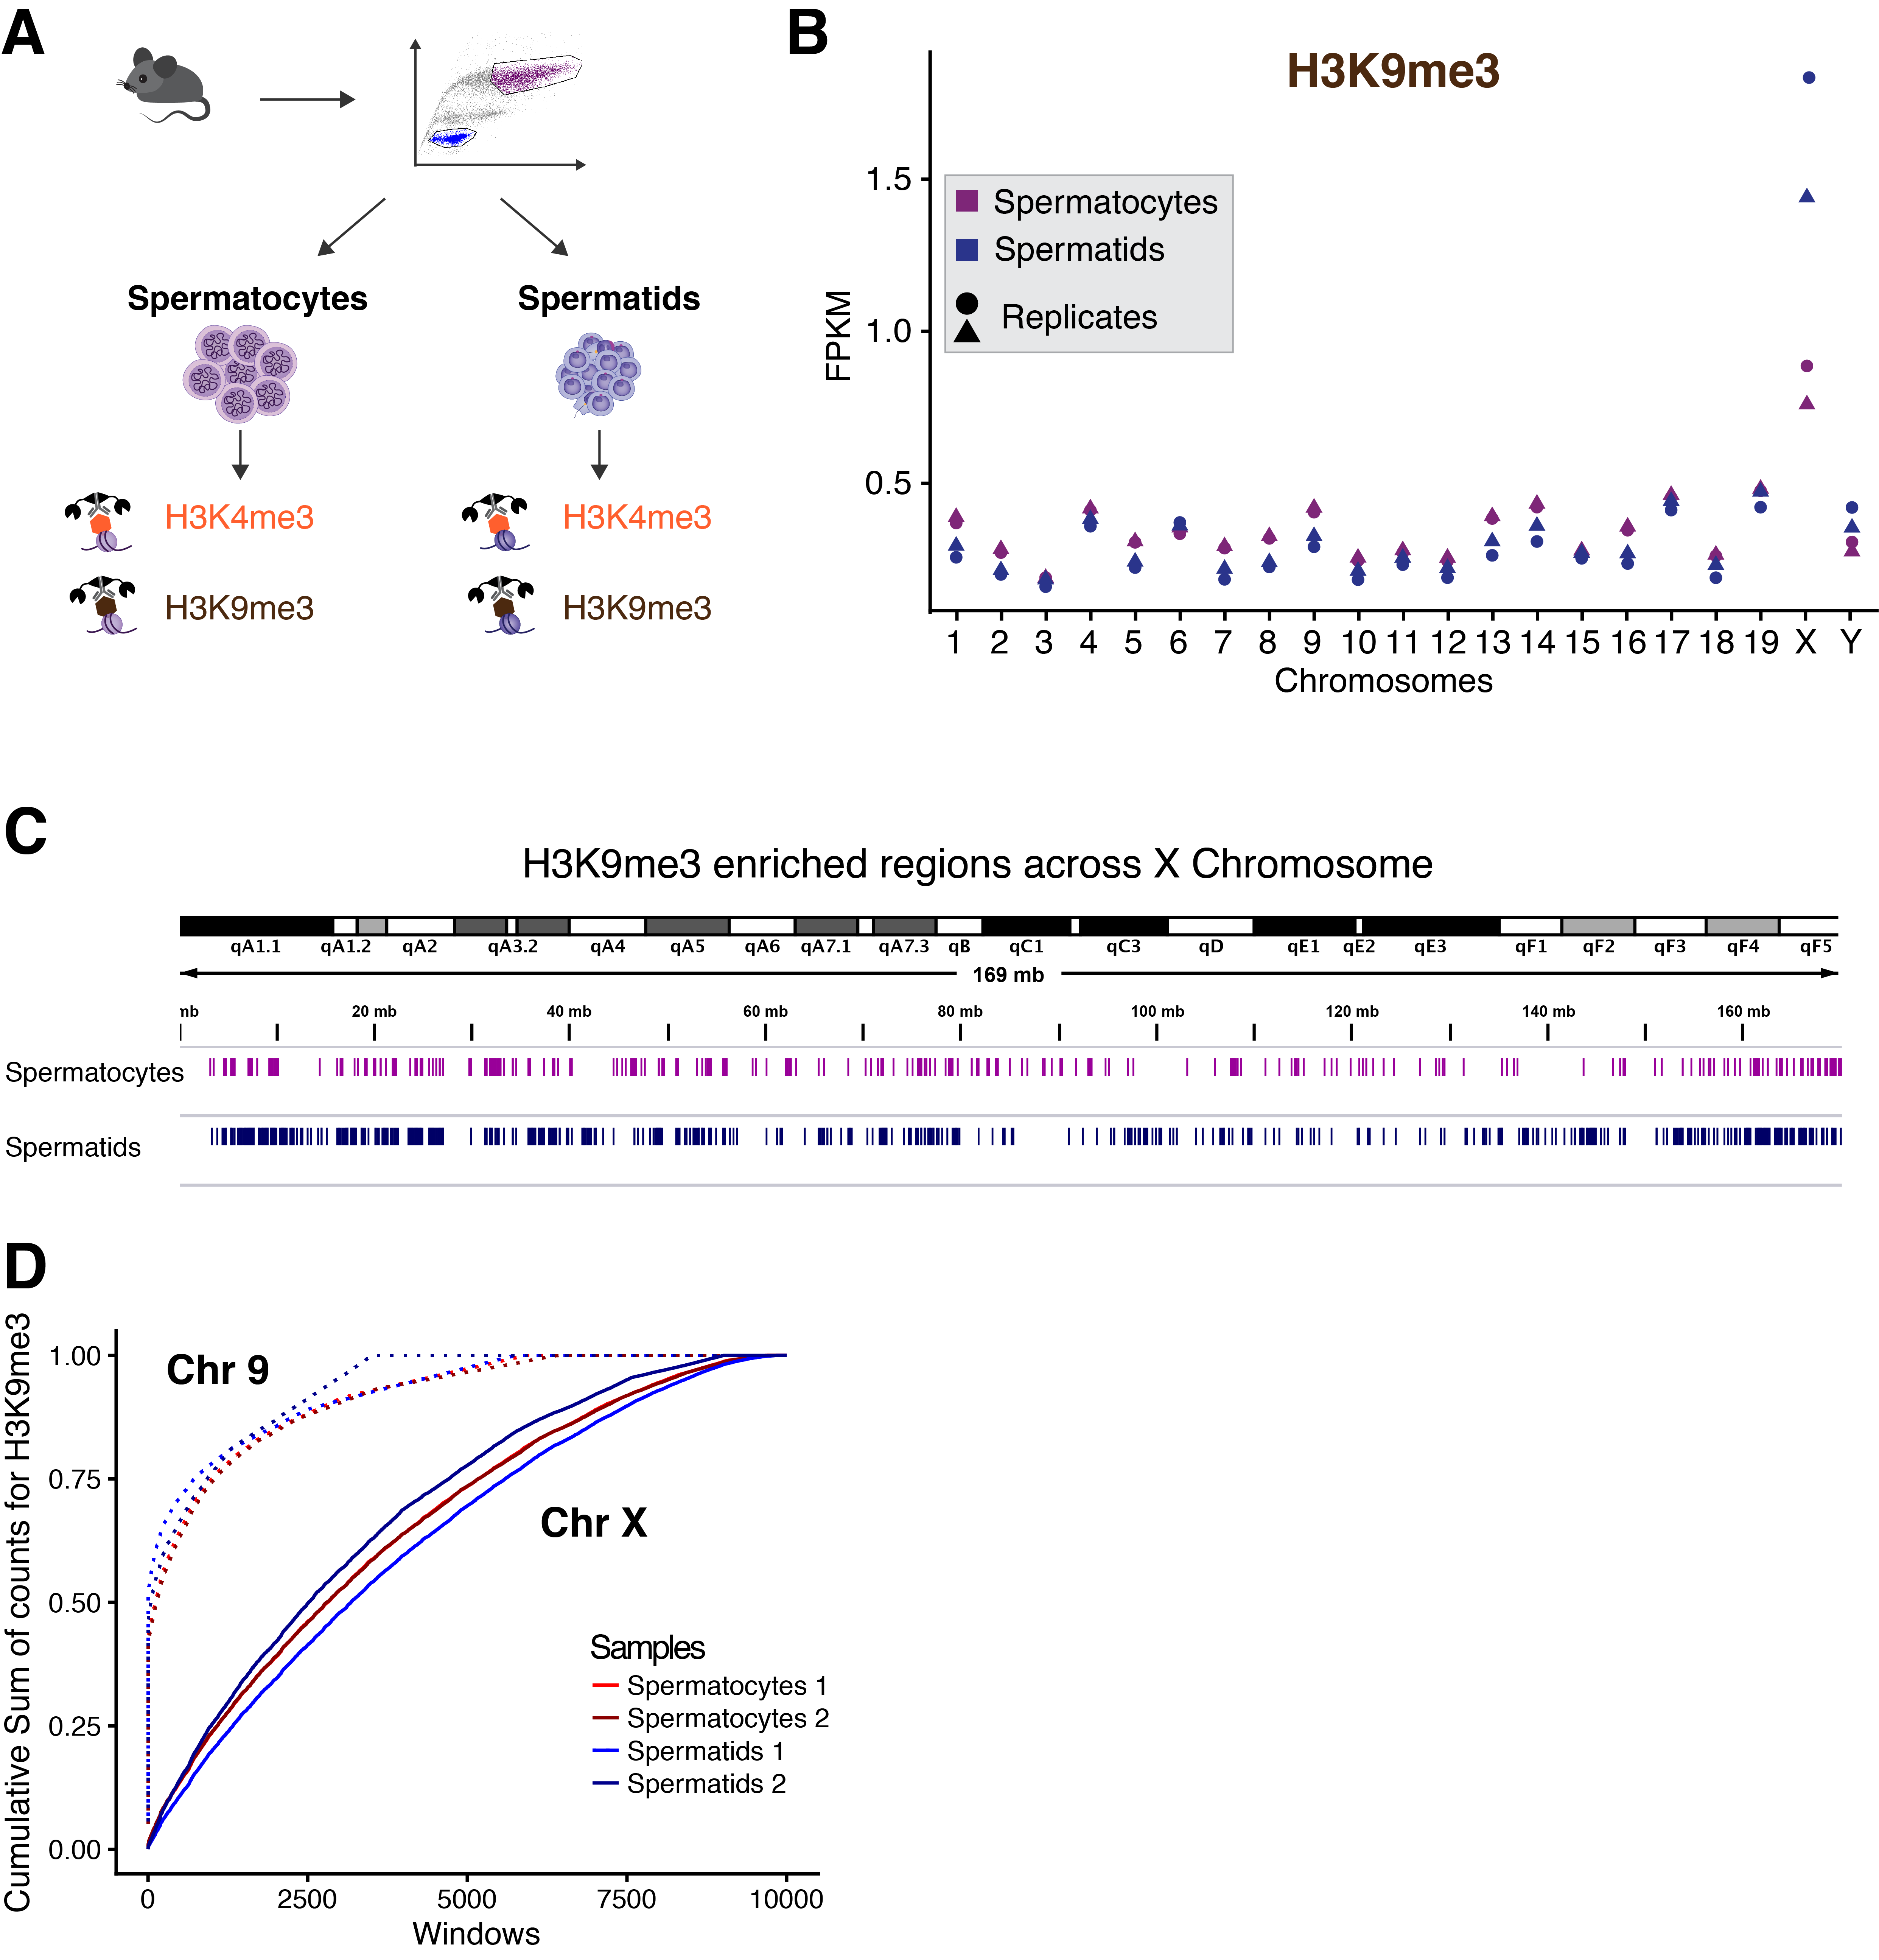
\includegraphics[width=\textwidth]{Fig_12.png}
\caption[ScDNA-Seq allows detection of SNVs and CNVs between individual cells]{\textbf{ScDNA-Seq allows detection of SNVs and CNVs between individual cells.}\\
Individual nuclei are captured in 96-well plates and directly lysed or fixated for multiplexing. Whole genome amplification (WGA) can be performed using MDA, MALBAC or SCOMP resulting in amplified genome segments. 
Depending on the biological question, whole genomes are either sequenced thoroughly to detect single nucleotide variants (SNVs) while shallow sequencing can be used to detect copy number variations (CNVs).}
\label{fig0:scDNA-Seq}
\end{figure}

\vspace{-5mm}

\subsubsection{Single-cell RNA sequencing}

Initial approaches to quantify mRNA abundance within single cells included targeted microfluidic-based single-cell \gls{RT-PCR} \citep{Warren2006} and whole-transcriptome read-outs of hand-picked cells \citep{Tang2009}. 
Methods for cell capture range from micromanipulation \citep{Grindberg2014} and laser capture microdissection \citep{Frumkin2008} as targeted methods with low throughput to  \gls{FACS} \citep{Hayashi2010, Dalerba2011, Jaitin2014}, microfluidics \citep{Trapnell2014, Treutlein2014} and microdroplets \citep{Klein2015, Macosko2015} as high-throughput approaches \textbf{(Fig.~\ref{fig0:scRNA-Seq})}. 
More broadly, microfluidic-based \gls{scRNA-Seq} approaches can be grouped into valve-, droplet- or well-based strategies \citep{Prakadan2017}. \\

A variety of scRNA-Seq protocols have been published that utilise different methods for mRNA \gls{RT}, \gls{cDNA} amplification and library preparation. 
All of these commonly used techniques for scRNA-Seq select and reverse transcribe mRNA (poly(A) tailing). 
The initial protocol introduced by Tang \textit{et al}, 2009 \citep{Tang2009} was improved by incorporating a template switching mechanism at the 5' end of the mRNA thus reducing the 3' sequencing bias present in previous methods \citep{Islam2011} (see below and \textbf{Fig.~\ref{fig0:scRNA-Seq}}). 
This \gls{STRT} method shows 5' bias in read mapping and was later modified for full-length transcript detection (SmartSeq \citep{Ramskold2012} and SmartSeq2 \citep{Picelli2013}). 
CEL-Seq \citep{Hashimshony2012} and CEL-Seq2 \citep{Hashimshony2016} use \gls{IVT} to linearly amplify cDNA prior to sequencing as opposed to exponential amplification in other techniques. 
Protocols for sequencing library preparation have been optimised for Illumina, SOLiD or PacBio sequencing \citep{Kolodziejczyk2015review}. \\

During scRNA-Seq, minute amounts of mRNA are captured and amplified generating a high degree of technical noise, which distorts quantification of true biological variability. 
To account for this, a set of external RNAs developed by the \gls{ERCC} \citep{Rna2005} can be added to the cell lysate. 
Based on the reads mapped to ERCC spike-ins, technical noise can be removed from total expression variability \citep{Brennecke2013, Vallejos2015BASiCS}. 
Another way to reduce noise derived from amplification biases in scRNA-Seq experiments is to tag each mRNA molecule with a \gls{UMI} \citep{Kivioja2011, Islam2014}.\\

One example of a commercially available platform that captures individual cells and performs lysis, reverse transcription and pre-amplification of cDNA is the Fluidigm\textsuperscript{\textregistered{}} C1 system. 
Individual cells are loaded into \glspl{IFC}, also termed "chips", that allows capturing of 96 to 800 cells. 
Depending on the size of the cells, this system offers chips with different capture well sizes. 
Each well can be microscopically inspected to differentiate between empty capture sites and single cells \citep{Kolodziejczyk2015review}. 
The C1 system uses the SMARTer\textsuperscript{\textregistered{}} chemistry to capture poly(A) mRNA with modified oligo(dT) primer. 
Next, the \gls{RTase} reverse transcribes from the 3' to the 5' end of the mRNA and adds non-templated deoxycytidines to the 3' end of the cDNA. The template-switch primer contains guanosines at its 3' end that base-pair with the deoxycytidines on the cDNA to create an extended template. 
The \gls{RTase} extends to the end of the template-switch primer. 
This produces single-stranded cDNA that contains the SMARTer tag sequence, the 3' end of the mRNA, the full-length transcript up to the 5' end of the mRNA, and the reverse complement of the SMARTer tag sequence. 
Amplification of this cDNA is performed by PCR on the chip \cite{Fluidigm2015}. After pre-amplification, the cDNA is collected and prepared for sequencing.\\

In parallel to extending scRNA-Seq protocols to robustly capture mRNA transcripts, efforts have been made to increase the throughput of this technology. 
Jaitin \emph{et al.}, 2014 introduced \gls{MARS-Seq} to sequence over 4000 cells of the mouse spleen. 
MARS-Seq captures cells in 384 well plates and labels transcripts of each cell with a combination of 2 random barcodes. 
This multiplexing strategy is performed using a liquid handling robot and cells can be pooled for sequencing library preparation which reduces costs and time effort \citep{Jaitin2014}. 
The first large-scale technique that captured tens of thousands of cells was introduced by Fan \emph{et al.} in 2015. 
Here, 10,000 cells were captured in a 100,000 microwell surface. 
Additionally, barcoded beads were loaded into the surface until saturation. 
This Cyto-Seq approach is similar to the more recent Seq-Well technology \citep{Gierahn2017}. 
Each bead is coated with barcodes containing a unique sequence, a bead-specific barcode, a UMI and a oligo(dT) primer. After cell lysis and mRNA capture, beads are pooled and cDNA synthesis can be performed prior to sequencing \citep{Fan2015}. 
In the same year, the inDrop and Drop-Seq technologies were introduced \citep{Klein2015, Macosko2015}. 
Both technologies use microfluidic platforms to merge droplets containing barcodes, lysis and reverse transcription reagents with droplets containing cells. 
Similar to the above described Cyto-Seq \citep{Fan2015}, after lysis and mRNA capture, droplets are pooled for sequencing. 
The main difference is that cell-specific barcodes in Drop-Seq are bound to beads and to a polyacrylamide mesh in inDrop.  

\begin{figure}[!h]
\centering
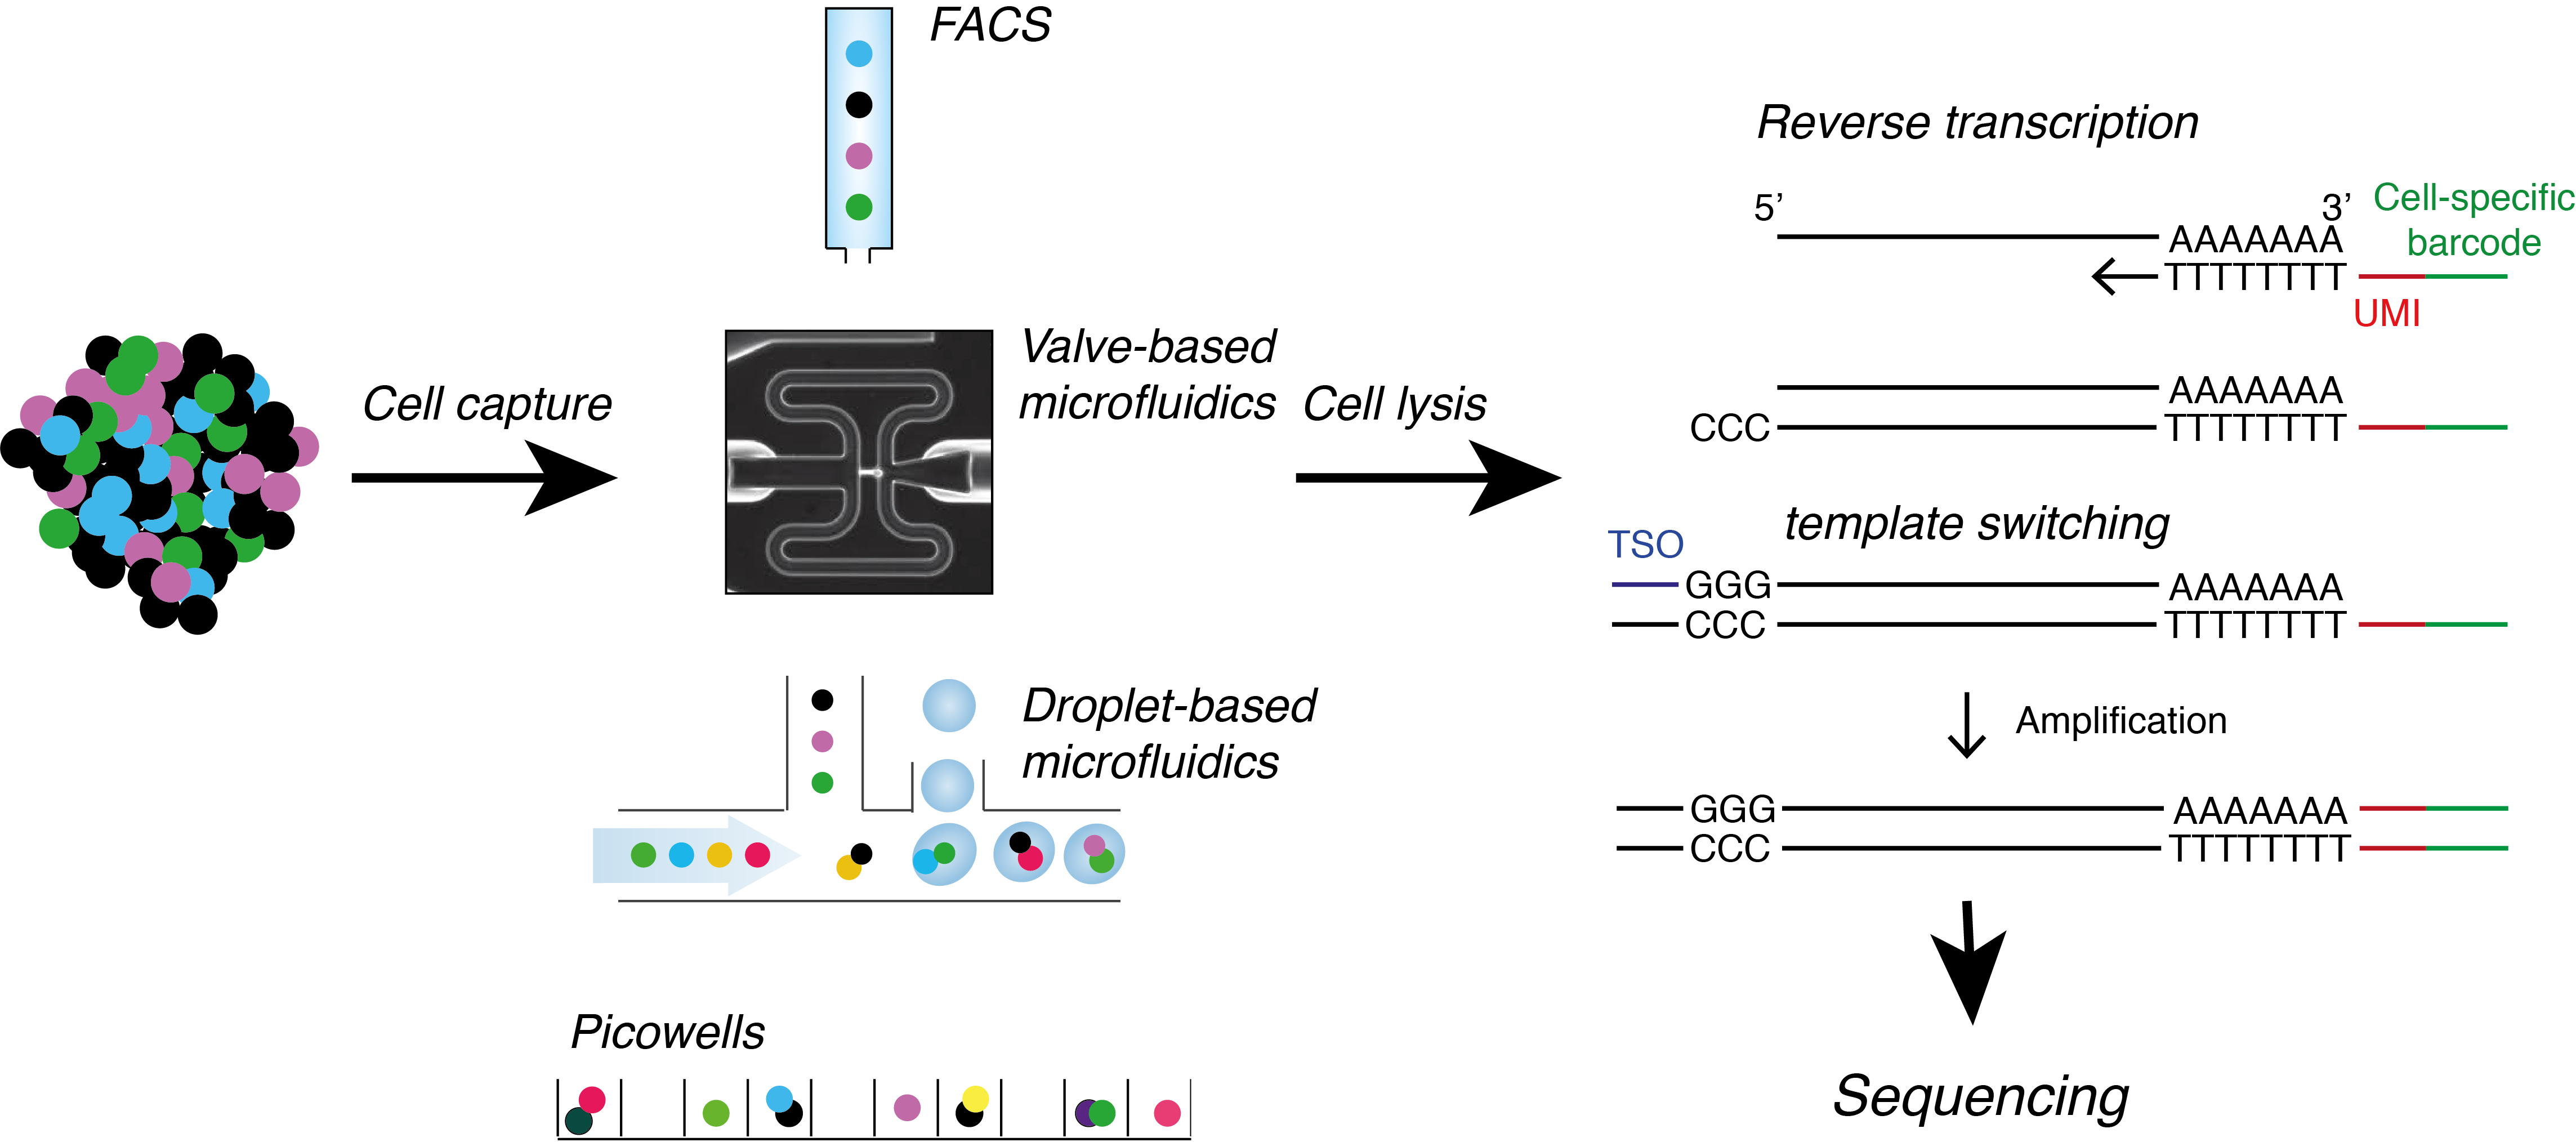
\includegraphics[width=0.9\textwidth]{Fig_13.png}
\caption[Workflow for scRNA-Seq technologies]{\textbf{Workflow for scRNA-Seq technologies.}\\
Single cell suspensions are obtained by tissue dissection and dissociation. 
Commonly used cell capture technologies include fluorescence-activated cell sorting (FACS), valve-based microfluidics (Fluidigm\textsuperscript{\textregistered{}} C1 system), droplet-based microfluidics (10X Genomics\textsuperscript{\textregistered{}} system), or picowells. 
After cell capture and lysis, poly(dT) oligos capture mRNA prior to reverse transcription. 
In the case of droplet-based cell capture, poly(dT) oligos are tagged with a unique molecular identifier (UMI) and a cell-specific barcode. 
\Gls{RT} generates cDNA from the template RNA. One strategy for RT is the template-switching protocol where the reverse transcriptase adds three cytidines at the 5' end of the template. 
A \gls{TSO} binds to the cytidines and allows amplification from the 5' end. 
After cDNA amplification, libraries are prepared for sequencing. For this, transposase degrades full length transcripts and Illumina sequencing primers are added (C1 system). 
In the case of the 10X Genomics system, the first read has been added next to the cell-specific barcode while the second read is added after cDNA fragmentation. This protocol shows a 3' bias.}
\label{fig0:scRNA-Seq}
\end{figure}

\newpage

10X Genomics\texttrademark{} has introduced a platform that uses these concepts to generate hundreds of thousands of \gls{GEM}. 
Around 80\% of generated oil droplets capture barcoded gel beads in 8 channels in parallel. 
Each barcode consists of a sequencing adapter and primer, a 14bp sequence from a pool of 750,000 barcodes, a 10bp UMI and a 30bp poly(dT) oligotide to capture poly(A) mRNA \citep{Zheng2017}. 
GEMs are fused with individual cells at a low concentration and cell lysis begins instantaneously. 
mRNA molecules are captured by the poly(dT) barcode and enzymes needed for \gls{RT} are released from the gel beads. 
After RT, each cDNA contains a transcript-specific UMI and a GEM-specific barcode making demultiplexing possible \textbf{(Fig.~\ref{fig0:scRNA-Seq})}. 
Barcoded cDNA is pooled for PCR amplification and library preparation \citep{Zheng2017}.\\

Methods that even further increased the throughput of scRNA-Seq include \gls{SPLiT-Seq} and sci-RNA-Seq. Similar to sci-DNA-Seq (see above) these technologies are based on combinatorial indexing of mRNA in fixed cells or nuclei. 
Sci-RNA-Seq tags transcripts during two rounds of indexing with UMIs and a combination of two cell specific barcodes \citep{Cao2017}.  
SPLiT-Seq on the other hand performs transcript tagging during 4 cycles adding 4 barcodes \citep{Rosenberg2018}. 
In that way, around 1 million cells can be uniquely labelled. At this stage the limiting factor is the sequencing depth needed to obtain high-resolution whole transcriptomes of each cell.	
These approaches as well as the recently developed \gls{DroNc-Seq} also allow sequencing mRNA from nuclei which is the preferred method for clinical samples, archived materials, and tissues that cannot be readily dissociated \citep{Habib2017}. 


\subsubsection{Single-cell epigenomics}

Single-cell epigenomic methods capture the chromatin state, histone modifications and DNA methylation state of individual cells and allow quantification of epigenetic variability across a population of cells \textbf{(Fig.~\ref{fig0:scEpigenomics})} \citep{Clark2016}. 
To observe methylation states of CpG motifs, \gls{scBS-Seq} involves the extraction of genomic DNA and cytosine to uracil bisulfite conversion prior to library preparation. 
5-methylcytosine remains intact during conversion \citep{Smallwood2014, Farlik2015}. 
The throughput of this approach was scaled up by combinatorial indexing of fixed nuclei similar to sci-DNA-Seq (i) prior to bisulfite conversion and (ii) during PCR amplification (sci-MET-Seq) \citep{Basque2017}. 
\Gls{scRRBS-Seq} enzymatically digests genomic DNA prior to bisulfite conversion. 
CpG-rich fragments can be enriched and amplified via ligated adapters before high-throughput sequencing \citep{Guo2013}. 
Extending the read-out of scBS-Seq and scRRBS-Seq, \gls{sc5hmC-Seq} captures the first oxidative product of CpG sites towards de-methylation and therefore cellular variation of methylation dynamics. 
Instead of bisulfite conversion, 5hmC sites are glucosylated before enzymatic digestion and adapter ligation \citep{Mooijman2016}. \\

To measure histone modifications or transcription factor binding dynamics at the single-cell level, digested chromatin from individual cells is tagged with barcodes prior to \gls{IP} during \gls{scChIP-Seq} \textbf{(Fig.~\ref{fig0:scEpigenomics})}. 
With this droplet-based method, variable chromatin signatures were detected across a population of ESCs based on the \gls{H3K4me2} \citep{Rotem2015}. 

\begin{figure}[!h]
\centering
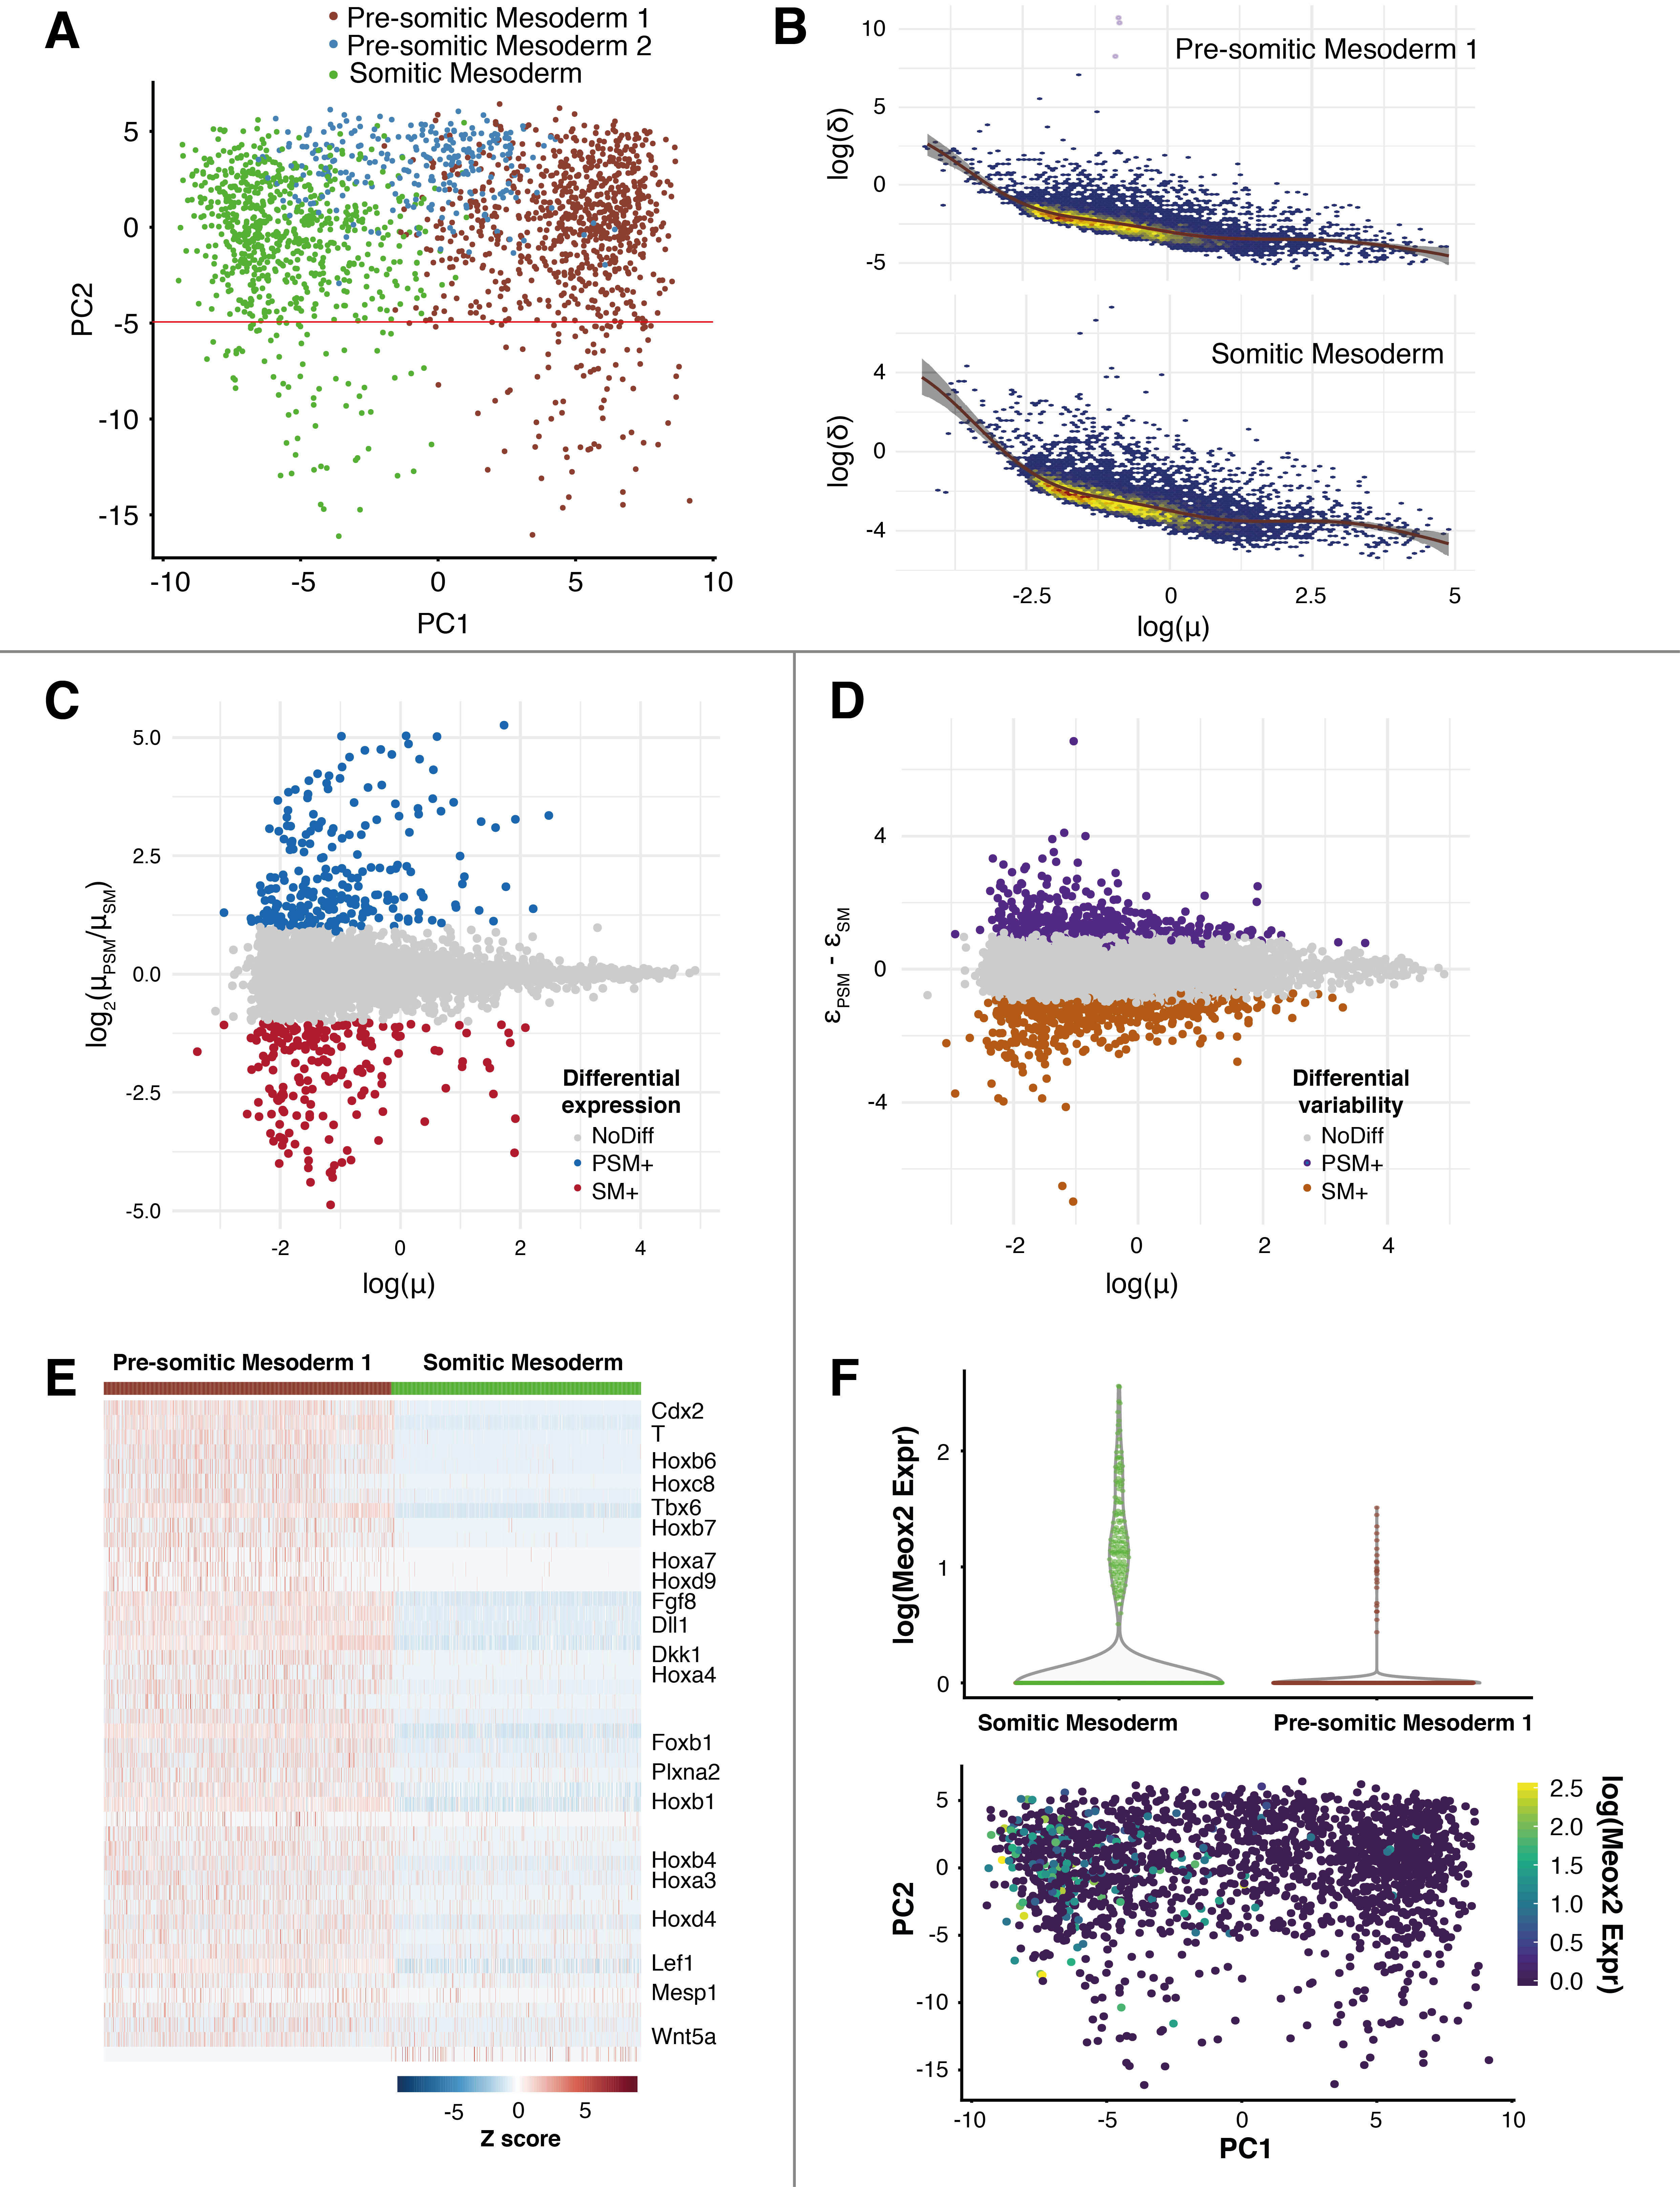
\includegraphics[width=\textwidth]{Fig_14.png}
\caption[Single-cell epigenomics to study chromatin structure and modifications]{\textbf{Single-cell epigenomics to study chromatin structure and modifications.}\\
Single-cell epigenomic technologies are used to study variation in DNA methylation, histone modifications, chromatin structure and nucleosome positioning across individual cells.}
\label{fig0:scEpigenomics}
\end{figure}

Other epigenomic approaches focus on estimating the patterns of open chromatin by measuring chromatin accessibility \textbf{(Fig.~\ref{fig0:scEpigenomics})}. 
\Gls{scATAC-Seq} captures individual cells on \glspl{IFC} before inserting sequencing adapters into accessible regions via the prokaryotic Tn5 transposase and pre-amplifiation. 
After library collection, cell-specific barcodes are added via a second round of PCR prior to sequencing \citep{Buenrostro2015}.  
Capturing cells in IFCs before barcoding limits the throughput to around tens or hundreds of cells at one time. 
Combinatorial indexing by tagging cells with barcodes in a two step process increases throughput for scATAC-Seq to thousands of cells \citep{Cusanovich2015}. 
An alternative approach to measure open chromatin involves the digestion of DNA with DNase I (Pico-Seq). 
The resulting small fragments undergo end-repair, adaptor ligation and PCR amplification in the presence of circular carrier DNA to avoid the loss of the minute amount of fragments \citep{Jin2015}. 
Similarly, nucleosome positioning can be detected by using the GpC-specific DNA \gls{MTase} M.CviPI to methylate cytosines of GpC motifs in regions where DNA is accessible. 
Individual cells are isolated and their DNA digested prior to bisulfite conversion. 
Patterns of methylated and unmethylated GpCs indicate the positioning of nucleosomes along the DNA \citep{Small2014}.\\

Single-cell technologies to study large-scale chromosome structure include \gls{DamID} \citep{Kind2015}, a method to identify lamina-associated domains, and single-cell \gls{HiC} \textbf{(Fig.~\ref{fig0:scEpigenomics})} \citep{Nagano2013}. 
Similar to sci-DNA-Seq, sci-RNA-Seq, sci-ATAC-Seq and sci-MET-Seq, sci-Hi-C uses multiplexing of fixated nuclei after digestion to insert (i) a biotinylated bridge adapter and later on a second adapter after lysis \citep{Ramani2017}. 
This technology allows the demultiplexing of thousands of cells after bulk-HiC-like processing. 

\subsubsection{Multi-omics approaches}

In recent years, some of the above described techniques were combined to measure transcriptomic, genomic, epigenomic and proteomic (“multi-omic”) features of single cells in parallel \citep{Macaulay2017}. 
The first approach for combinatorial \gls{DR-Seq} from the same cell amplifies genomic DNA and cDNA derived from reverse transcribed mRNA in one reaction step to avoid losses. 
After initial amplification, the sample is split to further process \gls{gDNA} and cDNA separately. 
PCR amplification increases the amount of gDNA while IVT amplifies cDNA prior to sequencing \citep{Dey2015}. 
An alternative approach, \gls{GT-Seq}, firstly separates gDNA and mRNA before whole-transcriptome and whole-genome amplification. 
Biotinylated oligo(dT) primers capture mRNA and are coupled to streptavidin coated beads. 
Once mRNA and gDNA is separated, the SmartSeq2 protocol is used to perform whole-transcriptome amplification while MDA or PicoPlex approaches can be used to amplify gDNA prior to sequencing \textbf{(Fig.~\ref{fig0:multiomics})} \citep{Macaulay2015}.\\

\begin{figure}[!h]
\centering
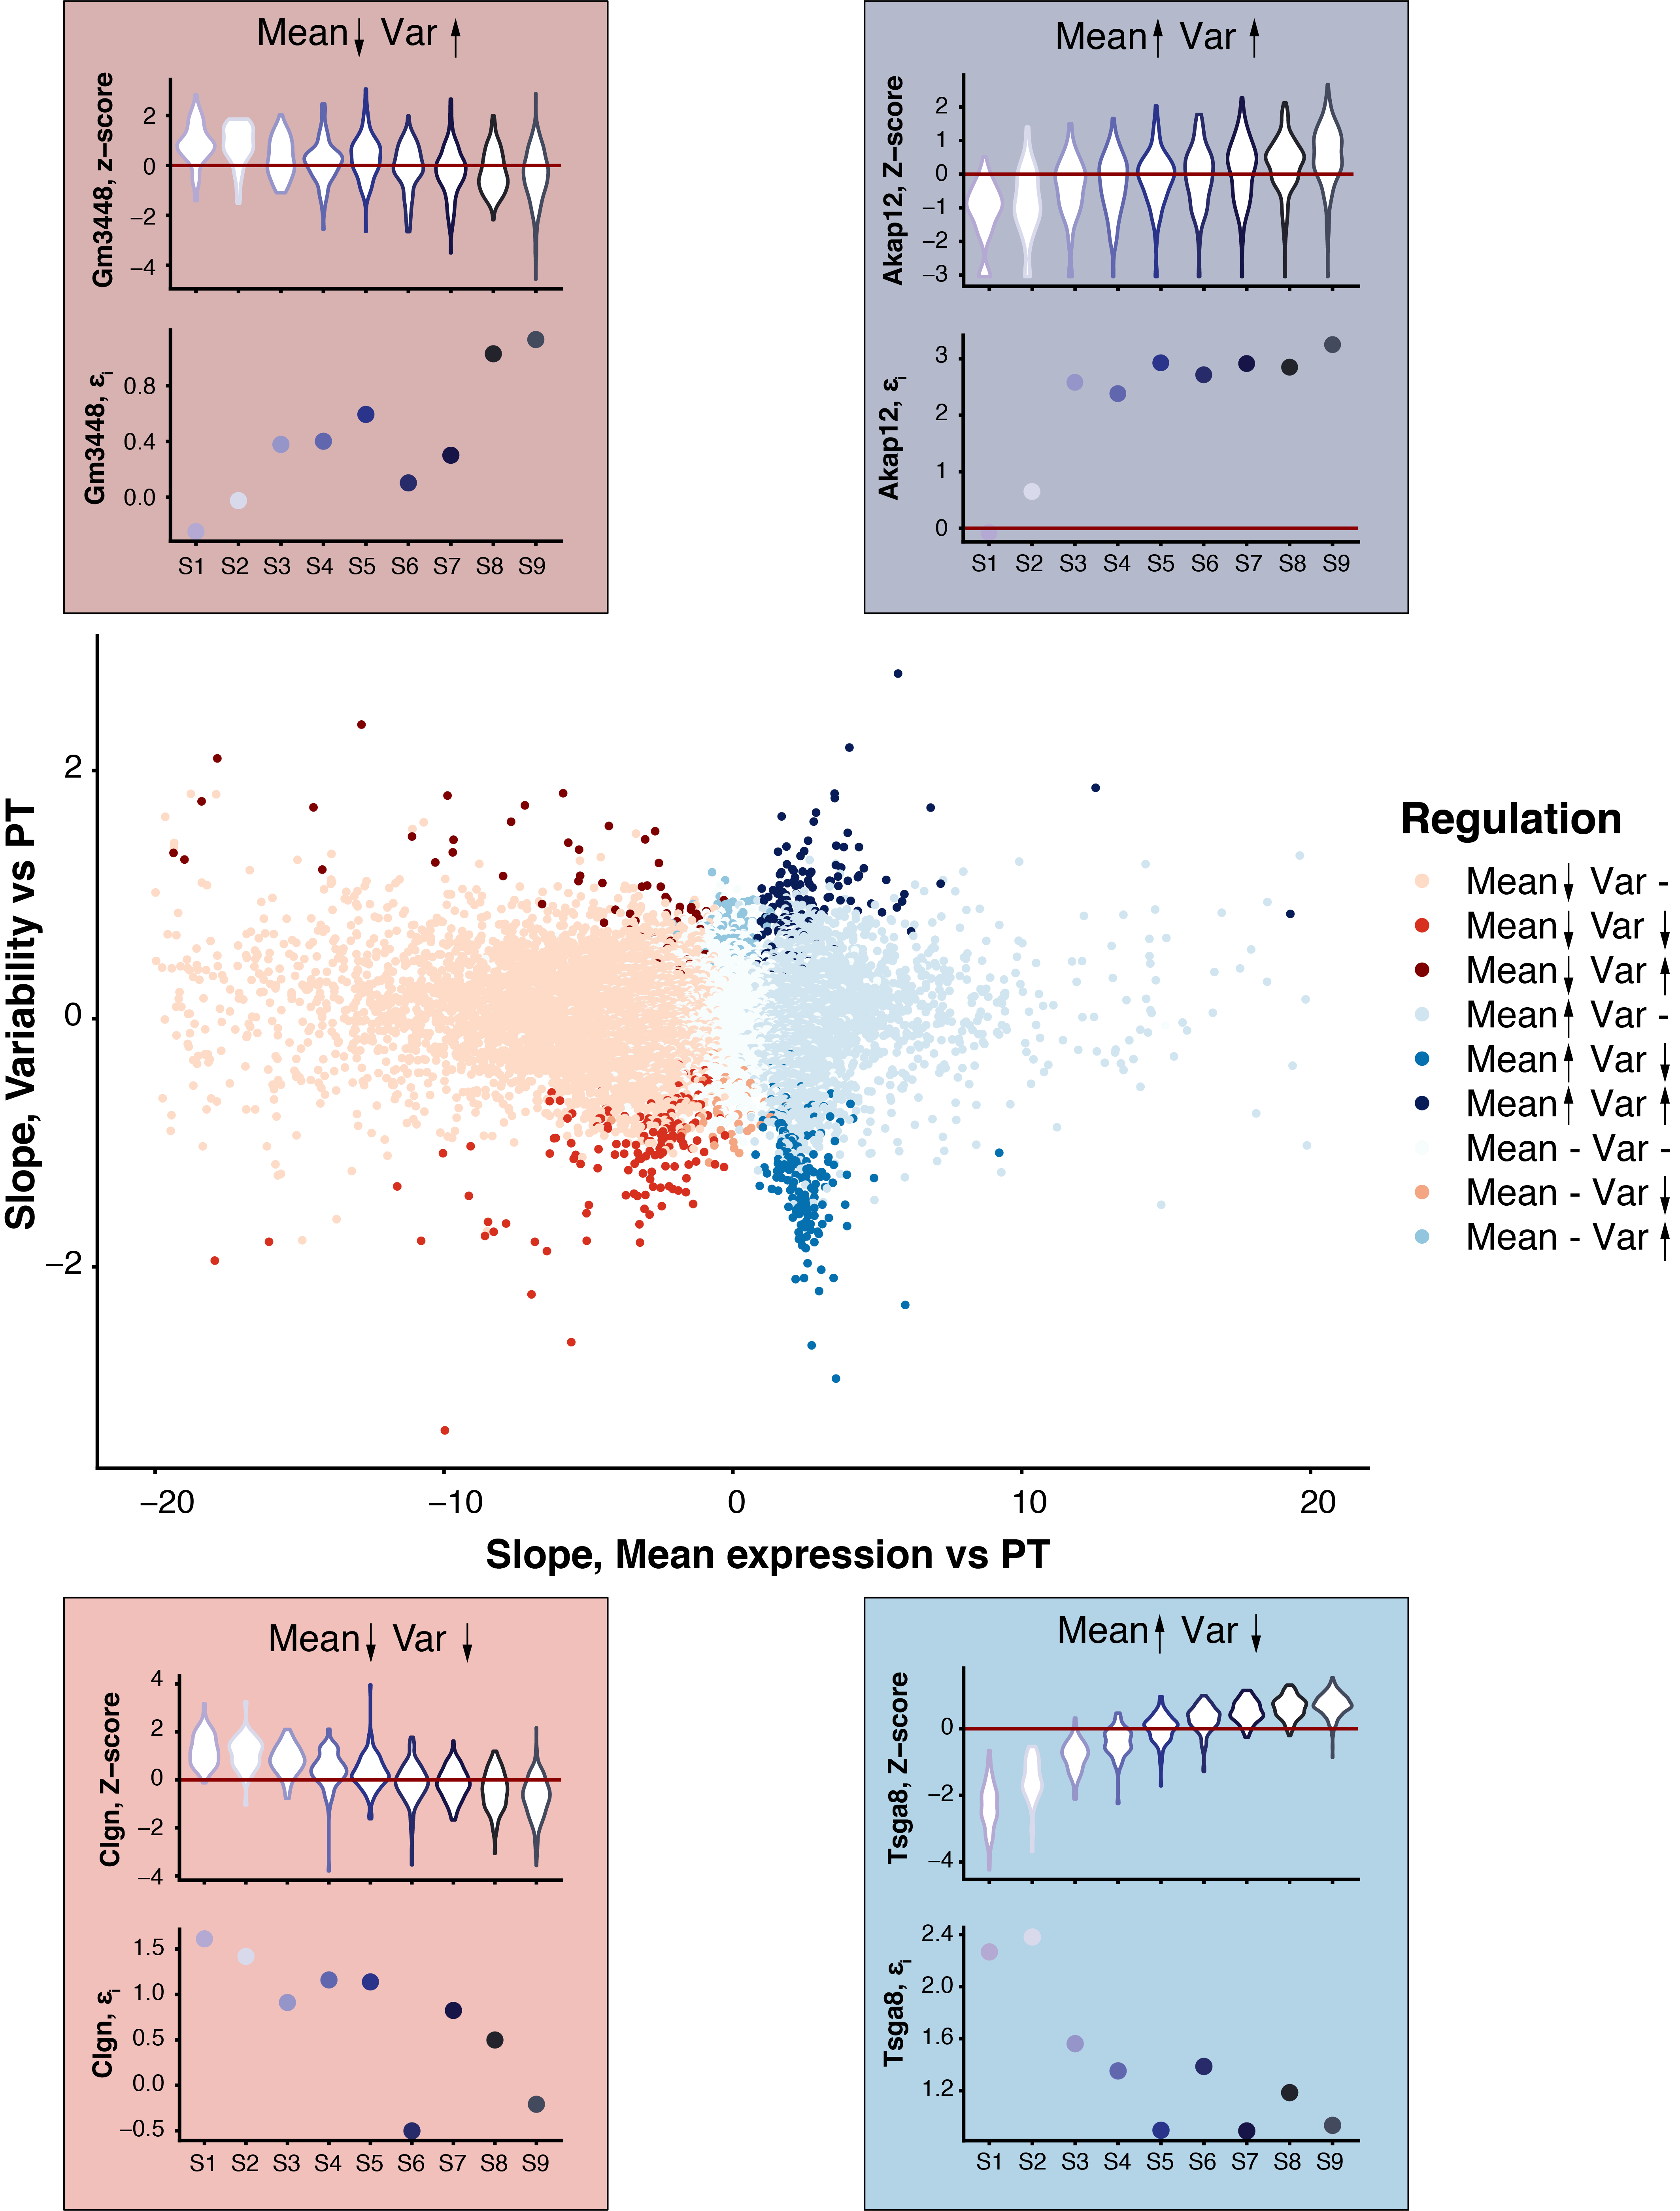
\includegraphics[width=\textwidth]{Fig_15.png}
\caption[Single-cell multi-omic approaches]{\textbf{Single-cell multi-omic approaches.}\\
Single-cell DNA and RNA-Seq either directly separates RNA and DNA or pre-amplifies both prior to separation. 
Measuring RNA and protein abundance from individual cells is done after physical separation followed by either oligonucleotide tagging of proteins or isotope tagging of RNA molecules. 
For methylome and transcriptome sequencing, DNA and RNA are separated prior to RNA sequencing and bisulfite conversion.}
\label{fig0:multiomics}
\end{figure}

Similarly, \gls{scMT-Seq} initially separates genomic DNA from mRNA. The scBS-Seq protocol is applied to isolated gDNA and is used to identify methylated CpG positions while mRNA was amplified via the SmartSeq2 protocol \citep{Angermueller2016a}. 
The scM\&{}T-Seq method has been extended to detect accessible chromatin regions in parallel to capturing methylated CpG sites and whole-transcriptome information. 
Prior to bisulfite conversion of gDNA, GpC sites are methylated by MTase in nucleosome sparse regions \textbf{(Fig.~\ref{fig0:multiomics})} \citep{Pott2017, Clark2018}.\\
 
Attempts have been made to capture $\sim$96 mRNAs in combination with proteins within individual cells. 
After cell lysis, samples are split to process mRNA and protein separately. 
mRNA is reverse transcribed and pre-amplified prior to \gls{qPCR} while oligonucleotide tagged antibodies bind to proteins. 
The free 3’-ends are complementary and can be extended by polymerisation to create a DNA reporter molecule. Similar to mRNAs, these molecules are detected using qPCR \citep{Darmanis2016}. 
This method has been scaled up by integration of droplet digital PCR \citep{Albayrak2016}. 
Alternatively, proximity ligation assay for RNA allows isotope tagging of RNA molecules, which are detected in parallel to proteins via mass cytometry \textbf{(Fig.~\ref{fig0:multiomics})} \citep{Frei2016}.

\subsection{Imaging approaches}

Similar to single-cell sequencing, RNA or protein imaging approaches quantify noise in biological systems \citep{Harton2017a}. 
Initial studies that addressed the extent of biological noise in bacterial populations used the expression of fluorescent proteins controlled by promoters of interest (reporter assays) to quantify expression noise \citep{Elowitz2002, Blake2003}. 
Later on, \gls{smFISH} was developed to capture variation in mRNA abundance across multiple cells \citep{Fang2013a, Lyubimova2013, Sanchez2013} and in whole organs \citep{Yang2014b}. 
Furthermore, the combination of fluorescently labelled proteins and smFISH allows the detection of co-variation between protein and mRNA levels within individual cells \citep{Taniguchi2011}. 
High-throughput automated smFISH of target RNAs in thousands of wells \citep{Battich2013} identified nuclear retention of RNAs as a mechanism to reduce cytoplasmic transcript variability \citep{Battich2015a}. 
Moreover, computerised image analysis and supervised machine learning extracts hundreds of cellular features from microscopy images and can therefore dissect variation of biological processes such as virus infection \citep{Snijder2009}.\\

The development of super-resolution microscopy allows detection of fluorophores that are spaced less than 100nm apart \citep{Sydor2015}. 
By combining \gls{STORM} and combinatorial labelling of RNA inside the cell, multiple transcripts from different genes can be visualised \citep{Lubeck2012}. 
This approach has been advanced to measure hundreds to thousands of RNA species per cell. 
\Gls{MERFISH} hybridises encoding probes to target RNAs prior to $N$ rounds of combinatorial labelling using fluorescently labelled read-out probes \textbf{(Fig.~\ref{fig0:MERFISH})}. 
MERFISH uses an encoding scheme that corrects for individual read-out errors based on a certain hamming distance between possible N-bit codes. 
Therefore, with 16 rounds of combinatorial labelling and a hamming distance of 4, 140 RNA species can be detected \citep{Chen2015}. A similar approach has been developed to profile spatial expression patterns in the mouse hippocampus (seqFISH) \citep{Shah2016}. 
By replacing the photobleaching step between consecutive rounds of combinatorial labelling with chemical cleavage and using multi-color imaging, the throughput of MERFISH can be increased \citep{Moffitt2016a}. 
Background fluorescence in tissue sections can be reduced by matrix-embedding of labelled RNA and cellular digestion \citep{Moffitt2016}.

\begin{figure}[!h]
\centering
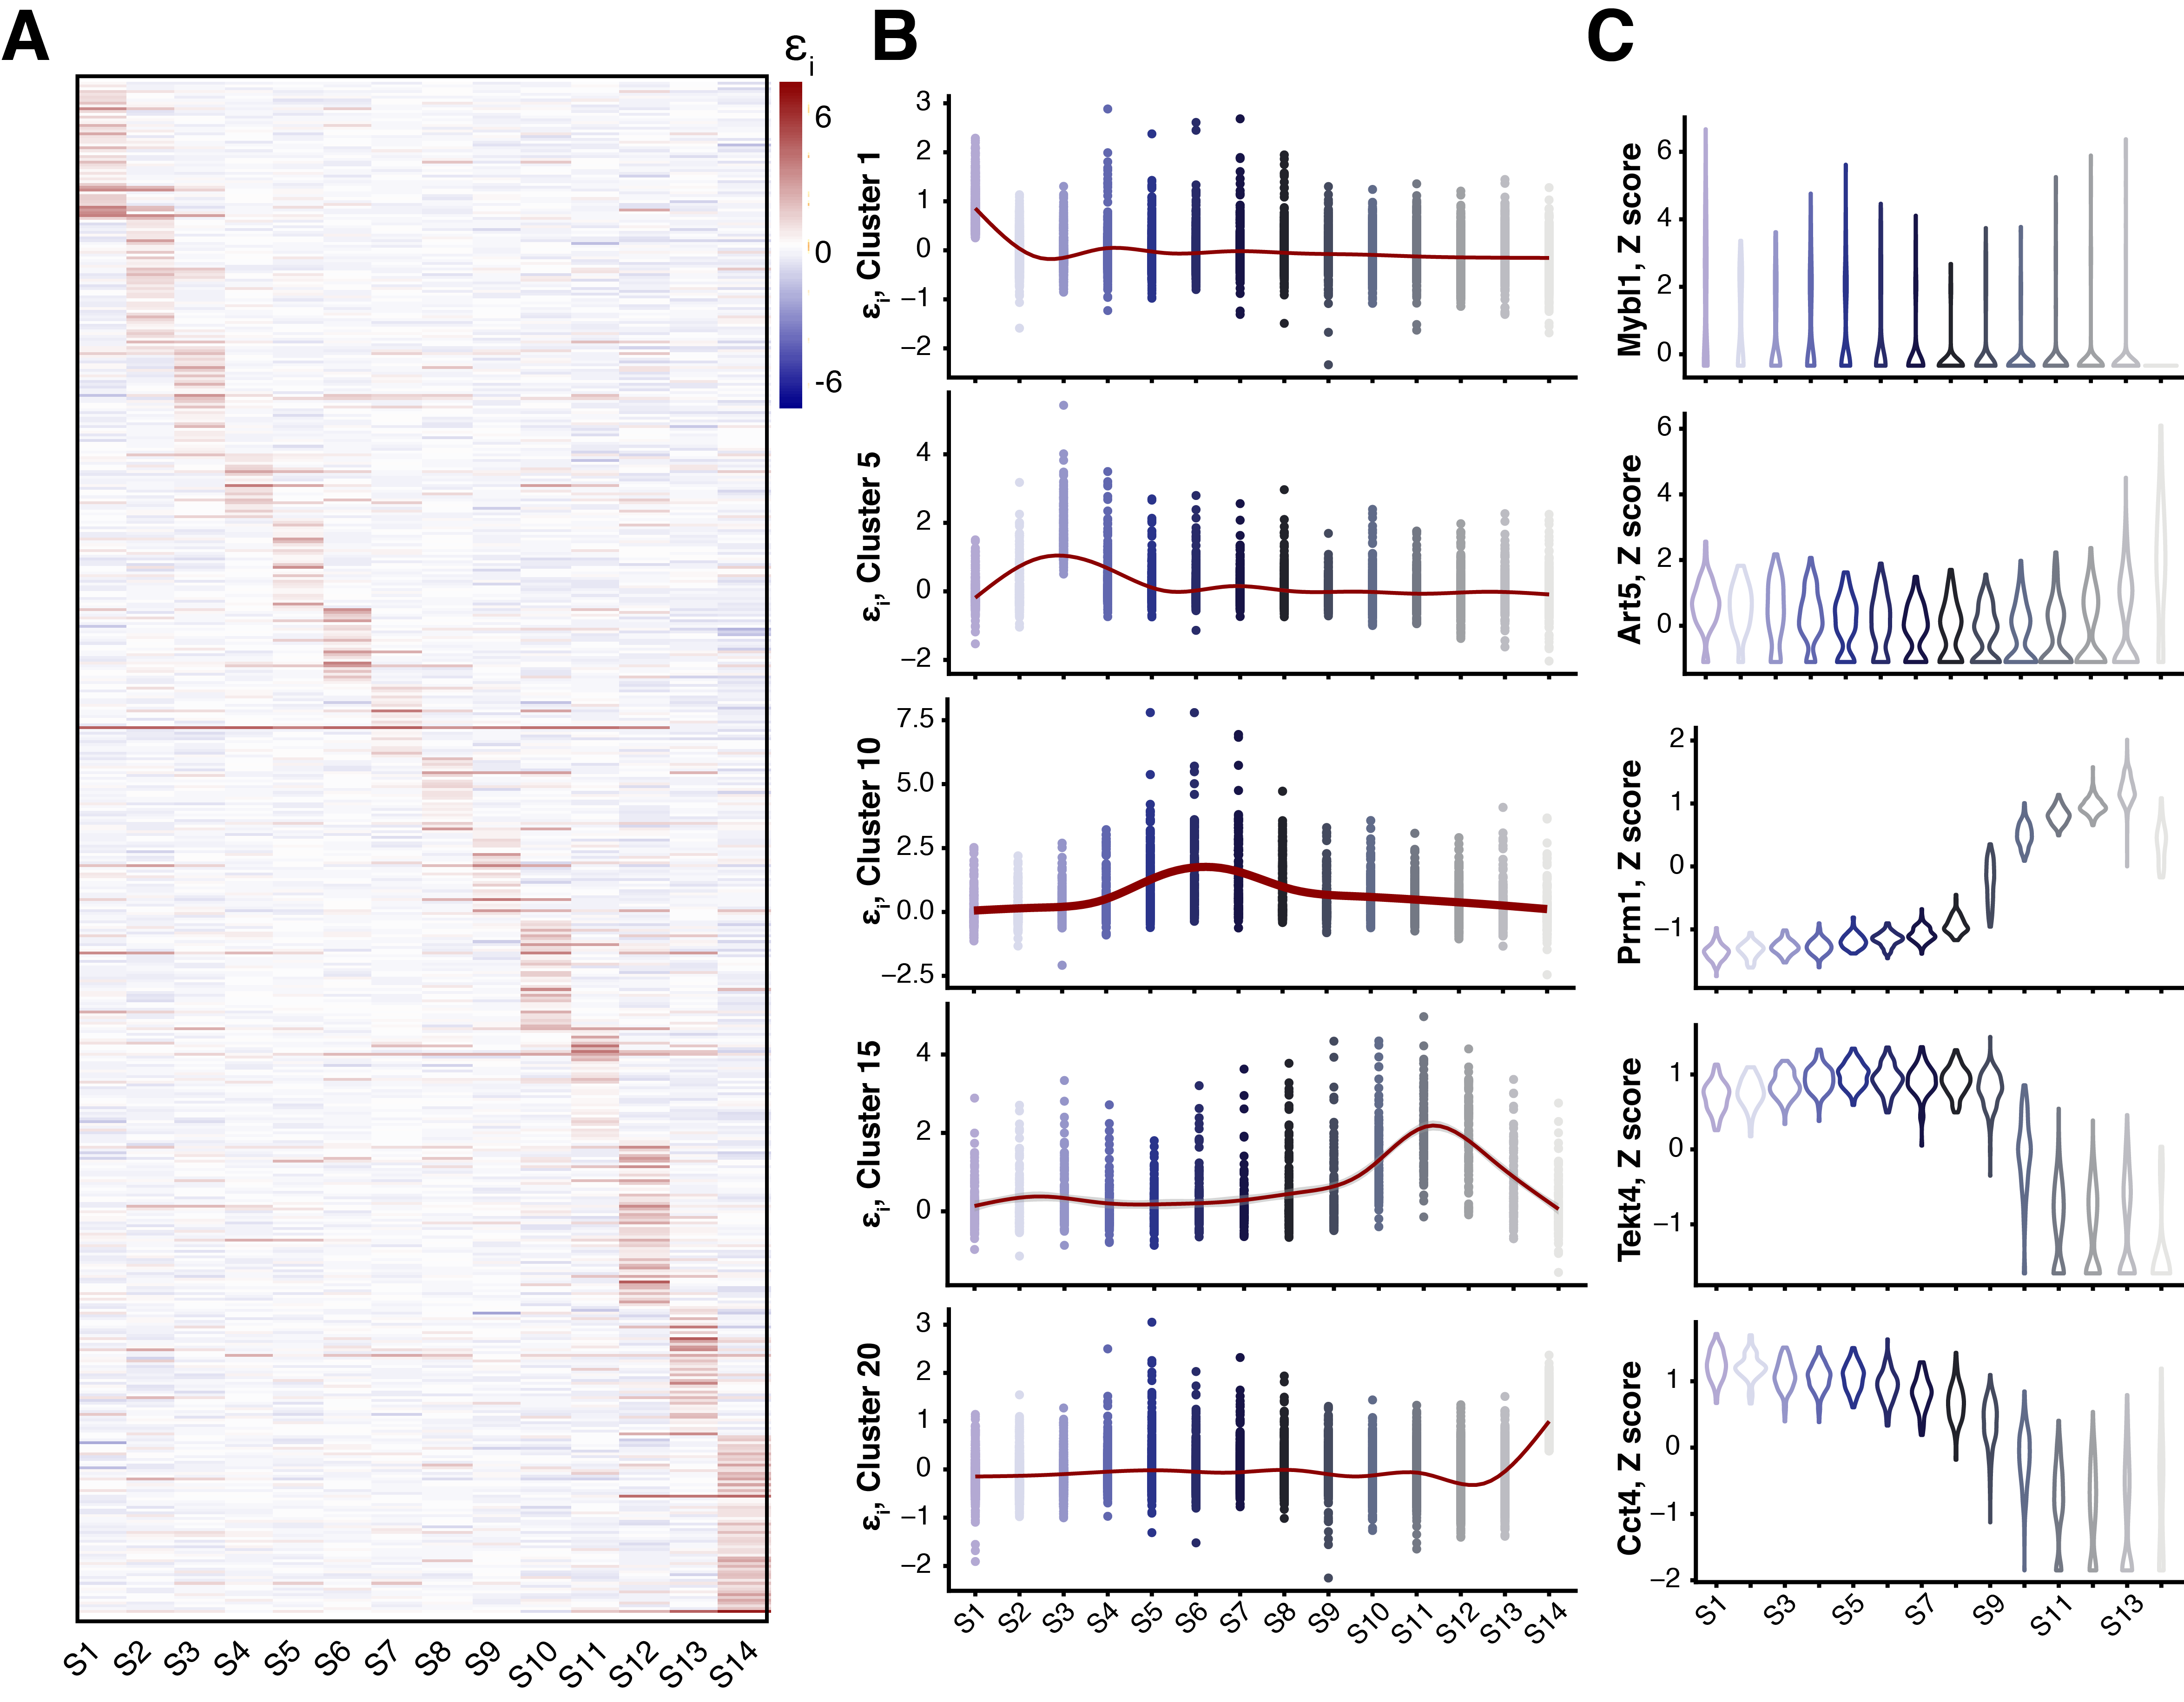
\includegraphics[width=\textwidth]{Fig_16.png}
\caption[MERFISH-type spatial transcriptomics]{\textbf{MERFISH-type spatial transcriptomics.}\\
Each transcript species is tagged with encoding probes that contain a sequence to recognise the RNA and multiple read-out sequences. 
During each hybridisation cycle, individual read-out probes hybridise with their specific sequences on the encoding probes. 
After multiple rounds of hybridisation and imaging, individual RNA transcripts can be decoded.}
\label{fig0:MERFISH}
\end{figure}

\subsection{Computational modelling and quantification}

Previous research focused on the derivation of mathematical frameworks to model expression dynamics in biological systems \citep{Tsimring2014}. 
In the simplest case, the central dogma of molecular biology states that mRNAs are synthesised from DNA at rate $k_m$ and proteins are translated from mRNAs at rate $k_p$. 
Furthermore, mRNAs are degraded at rate $\gamma_m$ and proteins at rate $\gamma_p$. 
In a noise-free system, this dogma leads to the following \textbf{deterministic}, first-order differential equation describing the number of mRNAs ($m$) and proteins ($p$) over time:

\begin{equation}
\frac{dm}{dt}=k_m-\gamma{}_mm,\quad \frac{dp}{dt}=k_pm-\gamma{}_pp
\end{equation}

\doublespacing
\noindent Steady-state transcript counts in this simple, two-stage system are defined as $\langle{}m\rangle{}=\frac{k_m}{\gamma_m}$  and protein abundance as $\langle{}p\rangle{}=\frac{k_mk_p}{\gamma_m\gamma_p }$. 
The variance for transcript and protein distributions are defined as: $\sigma^2=\langle{}m\rangle{}$ and $\sigma_p^2=\langle{}p\rangle{}\left[\frac{k_p}{\gamma_p+\gamma_m}+1\right]=\langle{}p\rangle{}\left[\frac{b}{1+\eta}+1\right]$, where $b=k_p/\gamma_m$  is the average number of proteins produced per transcript and $\eta=\gamma_p/\gamma_m$  \citep{Tsimring2014, Thattai2001}. 
mRNAs usually decay much faster than proteins. Therefore $\gamma_m\gg{}\gamma_p$ and $\sigma_p^2\cong\langle{}p\rangle{}\left[b+1\right]$ \citep{Thattai2001}. 
For this system, the mean translational burst size can be described as the Fano factor $\frac{\sigma_p^2}{\langle{}p\rangle}\cong{}b+1\approx{}b$ and burst frequency is captured by the inverse squared coefficient of variation $\frac{\langle{}p\rangle{}^2}{\sigma_p^2}\approx{}\frac{\langle{}p\rangle{}}{b}=\frac{k_m}{\gamma_p}=a$. The latter assumes that mRNAs are directly translated as soon as they are produced \citep{Friedman2006}.\\

\onehalfspacing
\noindent To account for stochasticity in this system, probabilistic expressions of the aforementioned equations have been described. 
The chemical master equation defines the time evolution of the probability of observing a system containing $m$ mRNAs and $p$ proteins at time point $t$:

\begin{align}
\frac{\partial{}P_{m,p}}{\partial{}t}&=k_m\left[P_{m-1,p}-P_{m,p}\right]+\gamma_m\left[(m+1)P_{m+1,p}-mP_{m,p}\right] \nonumber \\
&+k_pm\left[P_{m,p-1}-P_{m,p}\right]+\gamma_p\left[(p+1)P_{m,p+1}-pP_{m,p}\right]
\end{align}

\noindent The stationary probability distribution for this discrete representation of the master equation has the form of a negative-binomial distribution:

\begin{equation}
P_p=\frac{\Gamma(a+p)}{\Gamma(p+1)\Gamma(a)}\left(\frac{b}{1+b}\right)^p\left(1-\frac{b}{1+b}\right)^a
\end{equation}

\noindent where $a$ represents the burst frequency, $b$ the mean burst size and $\Gamma(n)$ the Gamma function \citep{Shahrezaei2008,Friedman2006,Tsimring2014}. 
Friedman \textit{et al.}, 2006 derived a stationary probability distribution from a continuous form of the chemical master equation \citep{Friedman2006}. 
This solution takes the form of a Gamma distribution:

\begin{equation}
P_p=\frac{1}{b^a\Gamma(a)}p^{a-1} e^{-p/b}
\end{equation}

\noindent This simple system has also been extended to incorporate the ON-OFF switching of promoters \citep{Jones2014, Shahrezaei2008}. 
Extensive modelling and quantification of mRNA and protein abundance in prokaryotic and eukaryotic cell populations confirmed this negative binomial (over-dispersed Poissonian) relationship between protein variance and abundance \citep{Ozbudak2002, Bar-Even2006}. 
The over-dispersion in protein abundance arises from biological noise ($\eta_{tot}$), which can be decomposed into intrinsic ($\eta_{int}$) and extrinsic ($\eta_{ext}$) contributions ($\eta_{tot}=\eta_{int}+\eta_{ext}$) \citep{Swain2002, Fu2016}. 
These components can be directly computed when using a two reporter system controlled by identical promoters \citep{Elowitz2002}. \\

Classic mathematical approaches to model transcriptional and translational dynamics use simplified assumptions for analytical tractability. 
Similar to the described translational bursting, transcriptional bursting as observed in eukaryotic cells \citep{Raj2006} leads to an over-dispersion in mRNA transcripts. 
Furthermore, while most models focus on single promoter dynamics, cases in which multiple promoters and competitor sites dilute TF binding have only recently been addressed \citep{Das2015a}. 
The assumption that translation from mRNA follows a first-order process was extended by using a hyperbolic Michaelis-Menten kinetic to model the translation process. 
This approach allows for continuous levels of ribosome occupancy on mRNAs \citep{VanDyken2017}. \\ 

While the models described above theoretically describe the expected distributions of proteins and mRNA across a population of cells, in practice, absolute measures (e.g.~transcript counts or fluorescence intensity) have to be used to quantify variation across a population of cells. 
In an early approach to model promoter kinetics from \gls{scRNA-Seq} data, Kim and Marioni, 2013 proposed a hierarchical Beta-Poisson model that relies on the switching dynamics of promoters between the "ON" and the "OFF" state ($k_{ON},k_{OFF}$) as well as the transcription rate $s$ and the decay rate $d$ \citep{Kim2013}. 
The model was formulated as follows:

\begin{align*}
X&|s,p\sim{}\text{Poisson}(sp)\\
p&|k_{ON},k_{OFF}\sim{}\text{Beta}(k_{ON},k_{OFF}),
\end{align*}

where $X$ is the transcript count per cell and $p$ a random effect dictated by promoter switching. 
Gene-specific inference was implemented as a Bayesian framework using Gamma distributions as priors for the hyper-parameters and Gibbs sampling to derive the posterior distributions of model parameters. 
The model indicates that RNAPII binding as well as histone modifications modulate burst size and burst frequency \citep{Kim2013}. \\

As an alternative, a variety of heterogeneity point estimates were computed to quantify biological noise. 
The variance $\sigma^2$, either calculated across all cells or across all expressing cells \citep{Shalek2014}, captures variability in RNA and protein abundance and scales linearly with mean expression $\mu$ \citep{Dey2015a}. 
The \gls{CV2} or the Fano factor are more widely used to measure heterogeneous RNA expression \citep{Brennecke2013, Jones2014} and protein abundance \citep{Newman2006}. 
Lowly expressed genes show higher levels of noise compared to highly expressed genes \citep{Brennecke2013}. 
Therefore, the CV$^2$ decreases with mean expression. 
To compare variability measures across different biological conditions where mean expression changes, regression approaches have been used to correct for the mean-variance relationship \citep{Kolodziejczyk2015cell, Fan2016}. 
Other approaches directly model biological variability as the excess in dispersion after removing technical noise \citep{Vallejos2015BASiCS}. 
Similar to the \gls{CV2} \citep{Brennecke2013} this over-dispersion measure decreases with increasing mean expression \citep{Vallejos2015BASiCS}. 
Moreover, heterogeneous expression can be captured by computing the Shannon entropy. Gene-specific entropy is defined as $H=-\sum_i{}p_i\log_2(p_i)$ where $p_i$ is the probability for a given gene being expressed in bin $i$. 
Binning across the expression counts can be done by choosing a fixed width \citep{Richard2016} or an adaptive width \citep{Stumpf2017}. 
Additionally, average pairwise distances between cells can capture increasing or decreasing heterogeneity in cell populations \citep{Mohammed2017}. \\ 

\newpage
%!TEX root = ../intro.tex
%******************************
%	 Other applications of scRNAseq
%*****************************

\section{General applications of scRNA-Seq in biology}

The following section outlines the broad spectrum of research fields that benefit from the development of scRNA-Seq technologies. Whole transcriptomic read-outs of individual cells allowed the in-depth characterisation of embryonic development, hematopoiesis, immune responses, allowed the detection of rare cell types and lead to new insights into disease progression including cancer development. 

\subsection{Atlas-type approaches}

Until recently, scRNA-Seq technologies were used to generate transcriptomes of less than a thousand cells to address specific questions in cellular systems such as cell-type heterogeneity, allele-specific expression or pseudo-temporal trajectories in gene expression \citep{Kolodziejczyk2015review}. With the development of scRNA-Seq technologies that massively increased the throughput of cell capture and data generation, cellular composition of whole tissues and organisms can be assayed. The largest of these so called "atlases" to date is the 10X Genomics\textsuperscript{\textregistered}{} brain dataset comprising 1.3 million cells from embryonic mice. I was generated using 133 libraries sequenced on 11 Illumina HiSeq\textsuperscript{\textregistered}{} 4000 flowcells \citep{Note2017}. This experiment has been performed to exemplify the applicability of the commercial 10X genomics platform to generate more than 10 billion transcriptomes of individual cells across the human body as envisioned by the Human Cell Atlas Consortium \citep{Regev2017}.\\

So far, examples of transcriptional atlases that comprise hundreds of thousands of cells are the mouse cell atlas, a thymus organogenesis atlas, an ageing lung atlas and the full characterisation of cell-types in \textit{C. elegans}. Similar to CytoSeq, Microwell-Seq was developed to capture more than 400,000 cells covering all mouse organ. This analysis reveals rare cell types, for example 2-cell-stage like mouse embryonic stem cells and allows the construction of a cross-tissue correlation network \cite{Han2018}. Similarly, the \emph{Tabula Muris} aimed at detecting all major cell type across 20 organs of the mouse. Here, the Tabular Muris Consortium decided to used droplet-based 3'-end scRNA-Seq and FACS-based full length transcript analysis to generate (i) a broad atlas and (ii) an in-depth characterisation of each tissue \citep{Quake2018}. Cao \emph{et al.}, 2017 generated more than 40,000 cells from the L2 stage \emph{C. elegans} using sci-RNA-Seq and identified nineteen distinct cell types and seven mixed cell types. Furthermore, this atlas allows the dissection of neuronal cell types that split across seven clusters \citep{Cao2017}. To study thymus development, Kernfeld \emph{et al.}, 2018 generated around 25,000 transcriptomes of individual cells from the embryonic thymus at E12.5, E13.5, E14.5, E15.5, E16.5, E17.5, E18.5, and P0. This experimental set-up resolves the temporal development of immune cell types such as T cells, myeolid cells, natural killer cells, innate lymphoid cells, and $\gamma{}\delta{}$ T cells as well as thymic epithelial cells \citep{Kernfeld2018}. Finally, to study the effect of ageing on a whole tissue, Angelidis \emph{et al.}, 2018 isolated 14,000 cells from lungs of young and old animals and found (i) and increase in transcriptional noise during ageing and (ii) altered transcriptional profiles of alveolar macrophages and type 2 pneumocytes \citep{Angelidis2018}.\\

The following paragraphs summarise scRNA-Seq applications which aimed at more targeted analysis of regulatory processes.

\subsection{Developmental biology}

For years, the development of new scRNA-Seq technologies and algorithms to perform data analysis uncovered driving factors in development and cell fate decisions \citep{Griffiths2018}. An early study during early mouse embryonic development identified that transcriptional differences between the two cells in the 2-cell stage embryo increase from the zygote to late 2-cell stage embryos. This is caused by an initial partitioning error where transcripts are unevenly distributed between the daughter cells and later on elevated by the onset of transcription coupled to transcriptional noise \citep{Piras2014, Shi2015a}. A reproducible distribution of transcripts in the first cell division was also detected by Biase \emph{et al.}, 2014 \cite{Biase2014}. These biases between cells at the 2-cell stage propagate to form transcription biases at the 4-cell stage to for the pluripotent inner cell mass or the extra-embryonic trophoectoderm \citep{Goolam2016, Shi2015a}. To obtain a more complete view on gastrulation in the mouse, Scialdone \emph{et al.} captured cells from the epiblast at E6.5 and mesodermal cells at E7.0, E7.5 and E7.75. The authors also sampled cells from \emph{Tal1} knock-out animals and showed that this transcription factor is the driving regulator for blood develeopment \citep{Scialdone2016}. \\

This year, large-scale scRNA-Seq studies profiled organogenesis in the mouse and zebrafish. Ibarra-Soria \emph{et al.} sampled more than 20,000 cells from E8.5 embryos following gastrulation and identified 20 major cell-types including different mesoderm lineages, neural progenitor cells, blood, gut and extra-embryonic cells. They further used this data to dissect gut formation and to find oscillating expression patterns during somitogenesis \citep{Ibarra-Soria2018}. Similarly, inDrop and Drop-Seq approaches were used to generate $\sim$7000 cells from \gls{Dmelanogaster} embryos at the onset of gastrulation todo{[rajewski reference]} or to generate more than 90,000 cells from the zebrafish embryo during the first day of development \citep{Wagner2018}.

In the last two years, experimental procedures were developed to track cells across multiple divisions termed "lineages". For this, the genome editing tool \gls{CRISPR}/\gls{Cas9} \citep{Jinek2012} was used to introduce so called "scares" at specific DNA sequences. In bacteria, the CRISPR/Cas system is used to degrade invasive DNA which involved a CRISPR RNA that recognizes the invading DNA and a Cas protein for degradation. For genome editing purposes, the \gls{CRISPR}/\gls{Cas9} uses guide RNAs to specific genomic sites and induces \gls{DSB}. Upon repair, insertions or deletion mutations are introduced that render a specific gene non-functional \citep{Zhang2014c}. The first approach to use the 	\gls{CRISPR}/\gls{Cas9} for scarring, \gls{GESTALT}, inserted an array of 10 \gls{CRISPR}/\gls{Cas9} with variable specificity into the genome of individual cells. Upon the expression of the Cas9 protein and the single-guide RNA, random scares are introduced into the genomic array. After days of growth genomic DNA was harvested and the array was sequenced to construct the relationship between individual cells \citep{McKenna2016}. This technology has been extended to a scRNA-Seq approach to capture the RNA together with the expressed \gls{CRISPR}/\gls{Cas9} array for cell-type detection and by a heat shock inducible system to start the scarring at later stages of development \citep{Raj2018}. Similar approaches uses multiplexed smFISH read outs to infer lineage relationship between individual cells \citep{Frieda2017} or tranposase-based insertion of a random 20mer sequence into the genome \citep{Wagner2018}.\\

One current challenge especially in the field of developmental biology is to obtain spatially-resolved whole-transcriptome read-outs of individual cells. The imaging technologies introduced above, MERFISH and SeqFISH, are capable of capturing single RNA molecules of thousands of genes across thousands of cells. Early approaches in the field of spatial transcriptomics employed spatial gene expression atlases to map isolated single cells back into the tissue of origin \citep{Achim2015a, Satija2015a}. A similar approach has recently been used to spatially locate cells isolated form the \gls{Dmelanogaster} embryo \todo{[rajewski reference]}. Moreover, Tomo-Seq was developed to sequence RNA extracted from slices of the zebrafish embryo. RNA was extracted from each slice into a tube and barcoded prior to sequencing. Matched histology and mathematical modelling was used to reconstruct the spatial expression patterns across the embryo \citep{Junker2014a}.

\subsection{Cell-type evolution} 

A smaller research field that uses scRNA-Seq approaches is evolutionary biology to understand the evolutionary origin of cell types. For this, non-model organisms such as \textit{Platynereis dumerilii} (annelid), \textit{Nematostella vectensis} (cniderian), \textit{Amphimedon queenslandica} (sponge), \textit{Mnemiopsis leidyi} (ctenophore) and \textit{Trichoplax adhaerens} (placozoan) are compared. All of these organisms (except annelids) are non-bilaterians and therefore evolutionary older than mouse and humans. As an example and part of an early project, we used the organism \textit{Platynereis dumerilii} to study diversification of cell-types in early bilaterian evolution. We detected cells from the apical neuroectoderm, the midgut, striated musculatrue, ciliated cells and non-apical blastopore cells. By assessing the transcriptional distance between these cell-types, we formulated a hypothesis of related cell-type families that originate from an ancesteral cell-type and are conserved during evolution \citep{Achim2018}.  \\

Seb\'e{}-Pedr\'o{}s \emph{et al.}, 2018 generated an single-cell genes expression atlas of adult and larval \textit{N. vectensis} using MARS-Seq. This dataset allowed the dissection of neuronal diversification and transcription factor regulatory programmes in this early sister group of bilaterians \citep{Sebe-Pedros2018}. The authors furthermore generated similar atlases of \textit{A. queenslandica}, \textit{M. leidyi} and \textit{T. adhaerens} and performed cross-species gene module analysis after cell-type identification. Co-regulation of cell-type-specific gene modules strongly diverged between the species except of few house keeping modules. Moreover, regulatory TF modules appear to be cell-type and species-specific \citep{Sebe-Pedros2018a}. These studies introduced scRNA-Seq as a powerful tool to study inter-species relationships of cell-types to dissect cell-type evolution. 

\subsection{Immunology}

The immune system has been extensively studied using scRNA-Seq to detect sub-cell-types, activation responses and to dissect the heterogenity of immune cells \citep{Proserpio2015, Satija2014}. White blood cells are broadly grouped into cells of the innate and adaptive immune system. Innate immune cells (dendritic cells, mast cells, macrophages, basophiles, \gls{NK} cells, neutrophils, eosinophil) are fast responders that represent the first line of defence in infections. The Adaptive immunity (B cells, CD4\plus{} and CD8\plus{} T cells) responds slower but installs an antigenic specificity and immune memory after infection \citep{Dranoff2004}. \\

\subsubsection{scRNA-Seq to study innate immunity}

Villani \emph{et al.}, 2017 used plate based scRNA-Seq to dissect the \gls{DC} and monocyte compartment of human \glspl{PBMC}. In general, DCs can be subdivided into CD11C\plus{} conventional DCs (CD141\plus{} and CD1C\plus{}) that activate CD4\plus{} and CD8\plus{} and interferon producing plasmacytoid DCs. Monocytes were classically subdivided into CD14\plus{} and CD16\plus{} cells. After analysing more than 2,400 DCs and monocytes, the authors expanded DCs to consist of 6 groups and detected conventional DC progenitor cells. Furthermore, they detected two new groups of uncharacterised monocytes \citep{Villani2017}. Shalek \emph{et al.}, 2014 used the C1 Fluidigm system to generate transcriptomes of more than 1700 primary mouse bone-marrow-derived DCs to study their activation response during \gls{LPS} stimulation. Within one hour of activation, early responding cells up-regulate \gls{Ifn}\textbeta{} and support the activation of surrounding cells via paracrine signalling. By isolating activated cells in individual chambers, the authors showed a decrease in the total number of activated cells after 4h stimulation with LPS. Furthermore, activated cells need autocrine stimulation to fully activate and IFN\textbeta{} secretion during the first hour of activation is the crucial trigger for full DC activation \citep{Shalek2014}. \\

Bj\"o{}rklund \emph{et al.}, 2016 performed targeted scRNA-Seq of Lin\textsuperscript{-}CD127\plus{} \glspl{ILC} and NK cells from tonsil tissue of adult humans using the SmartSeq2 protocol. They firstly identified the three major lineages of ILCs (ILC1, ILC2 and ILC3) and further assessed heterogeneity within the ILC3 population. Dissecting this rare cell-type allows a deeper understanding of immune regulation in humans \citep{Bjorklund2016}. 

\subsubsection{scRNA-Seq to study adaptive immunity}

An unbiased approach analysed $\sim$65,000 human \glspl{PBMC} and identified the major innate and adaptive immune cell-types. The authors further used droplet-based scRNA-Seq to study bone marrow mononuclear cells after hematopoietic stem cell transplant in order to treat \gls{AML}. The technology allowed the distinction between host and donor cells and the detection of residual AML cells in the host \citep{Zheng2017}. 

\subsection{Tissue function}

\todo{Mammary gland, liver}

\subsection{Cancer}

\todo{Avivs papers}
\newpage
%!TEX root = ../intro.tex
%******************************
%	 Bayesian approaches
%*****************************

\section{Bayesian approaches to model scRNAseq data}

As described above, expression counts in single-cell RNA-Seq data can be modelled as negative binomial distributed [ZINBABWE] while other approaches model these counts as log-normal distributed [BISCUIT, ZIFA]. This approach estimates cell and gene-specific parameters that can be used downstream for several tasks as normlization [Catas Nat Methods], clustering [ref], visualization [some latent space...] and imputation [MAGIC?], differential expression [e.g. MAST].   


\subsection{Scalability of Bayesian inference}

With the development of dropblet based approaches [Klein, Macosko] and multiplexed sequencing [Seqwell], scalability is important. 

Single-cell Variational Inference (scVI) 

scVI: transcriptomes of each cell are encoded through a non-linear transformation into a low-dimensional latent vector of normal random variables. latent representation is non-linearly transformed to generate a posterior distribution of model parameters based on a zer0-inflated negative binomial model. 

Zero-inflated negative binomial [Love 2014, Grun 2014, ZinBAWave]

The transcript count of gene $g$ in cell $n$ is modelled as zero-inflated negative binomial distributed:

\begin{align*}
x_{n,g} = 
 \left\lbrace
  \begin{aligned}
    &\textnormal{Poisson}(\phi_j\nu_j\mu_i\rho_{ij}), && i=1,...,q_0,j=1,...n;  \\ 
    &\textnormal{Poisson}(\nu_j\mu_i), && i=q_0+1,...,q,j=1,...,n,    	    
  \end{aligned}
\right.
\end{align*}

\subsection{Neural networks for modelling scRNA-Seq data}
 


\newpage
%!TEX root = ../intro.tex
%******************************
%	 Outline 
%*****************************


\section{Outline}

The overarching topic of this thesis is the quantification and interpretation of transcriptional noise as measured by scRNA-Seq. \textbf{Chapter 2} presents an initial experiment to study how  transcriptional noise effects the immune system. We see that transcriptional noise increases across multiple immune response genes during ageing which therefore could explain a disrupted immune response in older individuals. This finding has been published in following paper:

\begin{Abstract}
\hspace{-5mm} Celia P. Martinez-Jimenez$^\ast$, Nils  Eling$^\ast$, Hung-Chang Chen, Catalina A. Vallejos, Aleksandra Kolodziejczyk, Frances Connor, Lovorka Stojic, Tim F. Rayner, Michael J. T. Stubbington, Sarah A. Teichmann, Maike de la Roche, John C. Marioni, Duncan T. Odom. Ageing increases cell-to-cell transcriptional variability upon immune stimulation. \emph{Science}, 1436: 1433-1436, 2017, \\
($^\ast$ equal contributions) 
\end{Abstract}

Studying changes in variability between two conditions was restricted to genes that did not change in mean expression due to a strong confounding between variability and mean expression. In \textbf{Chapter 3}, I therefore extended the statistical framework from chapter 2 to correct for this confounding effect. This correction lead to (i) a stabilization of model parameters, (ii) expansion of the gene set that can be tested for changes in variability and (iii) a novel way of interpreting transcriptional dynamics. This project has been published as:

\begin{Abstract}
\hspace{-5mm} Nils Eling, Arianne C. Richard, Sylvia Richardson, John C. Marioni, Catalina A. Vallejos. \\
Robust expression variability testing reveals heterogeneous T cell responses. \emph{Cell Systems}, In press, 2018
\end{Abstract}

The extended model offers the unique opportunity to study changes in variability across multiple cell types even when mean expression changes. In \textbf{Chapter 4}, I apply the newly developed model to test changes in variability over pseudotime. For this, droplet-based scRNA-Seq data of mouse spermatogenesis was used to dissect the transcriptional dynamics during this developmental process. Parts of the study are available online as:

\begin{Abstract}
\hspace{-5mm} Christina Ernst$^\ast$, Nils Eling$^\ast$, Celia P. Martinez-Jimenez, John C. Marioni, Duncan T. Odom. Staged developmental mapping and X chromosome transcriptional dynamics during mouse spermatogenesis. \emph{bioRxiv}, 2018, ($^\ast$ equal contributions)
\end{Abstract}

Finally, I will discuss current challenges in modelling transcriptional noise from scRNA-Seq data and experimental strategies to modulate expression variability.

\newpage

\section{Other contributions}

Contributions to papers that are not discussed in this thesis are as follows:\\

\begin{Abstract}
Kaia Achim$^\ast$, Nils Eling$^\ast$, Hernando Martinez Vergara, Paola Yanina Bertucci, Jacob Musser, Pavel Vopalensky, Thibaut Brunet, Paul Collier, Vladimir Benes, John C. Marioni, Detlev Arendt. Whole-Body Single-Cell Sequencing Reveals Transcriptional Domains in the Annelid Larval Body. \emph{Molecular Biology and Evolution}, 35: 1047-1062, 2018, ($^\ast$ equal contributions)
\end{Abstract}

\begin{Abstract}
Christina Ernst, Jeremy Pike, Sarah J. Aitken, Hannah K. Long, Nils Eling, Lovorka Stojic, Michelle C. Ward, Frances Connor, Timothy F. Rayner, Margus Lukk, Robert J. Klose, Claudia Kutter, Duncan T Odom. Successful transmission and transcriptional deployment of a human chromosome via mouse male meiosis. \emph{eLife}, 5: e20235, 2016 
\end{Abstract}
